%%% Macros that should probably be defined before

% h-propositions
\newcommand{\anhprop}{a mere proposition\xspace}
\newcommand{\hprops}{mere propositions\xspace}

%%% Local macros

% Subuniverse
\renewcommand{\P}{\ensuremath{\mathsf{P}}\xspace}
% Reflector, projection and extension in an arbitrary reflective subuniverse
\newcommand{\reflect}{\mathsf{r}}
\newcommand{\project}{\mathsf{p}}
\newcommand{\ext}{\mathsf{ext}}

\chapter{Homotopy theory}
\label{cha:homotopy}

In this chapter, we develop some homotopy theory within HoTT.  

\section{Overview}

We begin with a very brief summary of classical homotopy theory,
homotopy theory in $\infty$-groupoids, and homotopy theory in HoTT.

\subsection{Classical homotopy theory}

\emph{Topology} is the study of spaces up to continuous deformation.
\emph{Algebraic topology} is the use of tools from abstract algebra,
like group theory, to tell whether two spaces are the same.  As a first
cut, we can say that two spaces are "the same" when there is an
homeomorphism between them (continuous maps back and forth that compose to
the identity), though we will refine this later.  For example, one basic
construction in algebraic topology is the \emph{fundamental group} of a
space: Given a space $X$ and a point $x_0$ in it, one can (almost---see
below) make a group whose elements are loops at $x_0$ (paths from $x_0$
to $x_0$), with the group operations given by the identity path
(standing still), path concatenation, and path reversal.  Isomorphic
spaces have the same fundamental group, so fundamental group can be used
to tell two spaces apart: if $X$ and $Y$ have different fundamental
groups, they are not isomorphic.  Thus, the fundamental group is an
algebraic invariant that provides global information about a space,
which complements the local information provided by notions like
continuity.  For example, the torus locally looks like the sphere, but
has a global difference: it has a hole in it.  One way to see this is to
observe that the fundamental group of the sphere is trivial, but the
fundamental group of the torus is not.

To explain why this is so, we need to be a little more precise about
what the fundamental group is.  Consider a space $X$ with a path $p$
from $x$ to $y$.  Then there is an inverse path $\opp p$ from $y$ to
$x$.  Concatenating $p$ with $\opp p$ (written $p \ct \opp p$) gives a
path from $x$ to $x$, which should be the same as the identity path
(witnessing one of the inverse cancellation laws of a groupoid).
However, in topology, a path $p$ in $X$ is represented as a continuous
map from the interval $[0,1]$ into $X$, where $p(0) = x$ and $p(1) =
y$---think of the interval as "time" and $p$ as giving the point on the
path at each moment in time.  Under this definition, $p \ct \opp p$
(which walks from $x$ to $y$, and then back along the same route, as
time goes from $0$ to $1$) is not literally the same as the identity
path (which stays still at x at all times).  So loops don't actually
form a group!

The way to fix this is to consider the notion of \emph{homotopy between
paths}. Because $p \ct \opp p$ walks out and back along the same route, you know
that you can continuously shrink $p \ct \opp p$ down to the identity path---it
won't, for example, get snagged around a hole in the space.  Formally, a
homotopy between functions $f, g : X \rightarrow Y$ is a continuous map 
$h : [0,1] \times X \rightarrow Y$ such that $h(0,x) = f(x)$ and $h(1,x) = g(x)$.  In the specific case
of paths $p$ and $q$, which, remember, are represented by maps $[0,1] \rightarrow X$, a
homotopy is a continuous map $h(t,x) : [0,1] \times [0,1] \rightarrow X$, such that
$h(0,x) = p(x)$ and $h(1,x) = q(x)$.  That is, it's the image in $X$ of a
square that fills in the space between $p$ and $q$.  Homotopy is an
equivalence relation, and operations like concatenation, inverses,
etc., respect it.  Moreover, the homotopy equivalence classes of loops in
$X$ at $x_0$ (where two loops $p$ and $q$ are equated when there is a \emph{based}
homotopy between them, which is a homotopy $h$ as above that additionally
satisfies $h(t,0) = h(t,1) = x_0$ for all $t$) do form a group: while $p \ct \opp p$
is not equal to the identity, it is homotopic to it!  So, we can fix up
the above definition of the fundamental group of a space by defining it
to be the group of loops modulo homotopy.

Returning to the example, we can see that the sphere is different from
the torus because the fundamental group of the sphere is trivial (the
one-element group), but the fundamental group of the torus is not.  The
intuition is that every loop on the sphere is homotopic to the identity,
because its inside can be filled in.  In contrast, a loop on the torus that
goes around the donut's hole is not homotopic to the identity, so there
are non-trivial loops.

The fundamental group, which is written $\pi_1(X,x_0$), is the first in
a series of \emph{homotopy groups} that provide additional information
about a space.  Fix a point $x_0$ in $X$, and consider the constant path
$\refl{x_0}$.  Then the homotopy classes of homotopies between $\refl{}$ and itself form a
group $\pi_2(X,x_0$), which tells you
something about the two-dimensional structure of the space.  Then
$\pi_3(X,x_0$) is the group of homotopy classes of homotopies between homotopies, and so on.
One of the basic questions that algebraic topologists consider is
\emph{calculating the homotopy groups of a space $X$}, which means
giving a group isomorphism between $\pi_k(X,x_0)$ and some more direct
description of a group (e.g., by a multiplication table or
presentation).  Somewhat surprisingly, this is a very difficult
question, even for spaces as simple as the spheres.  Here is a chart
that lists the low-dimensional homotopy groups of the low-dimensional
spheres.

%% FIXME: recreate table in TeX
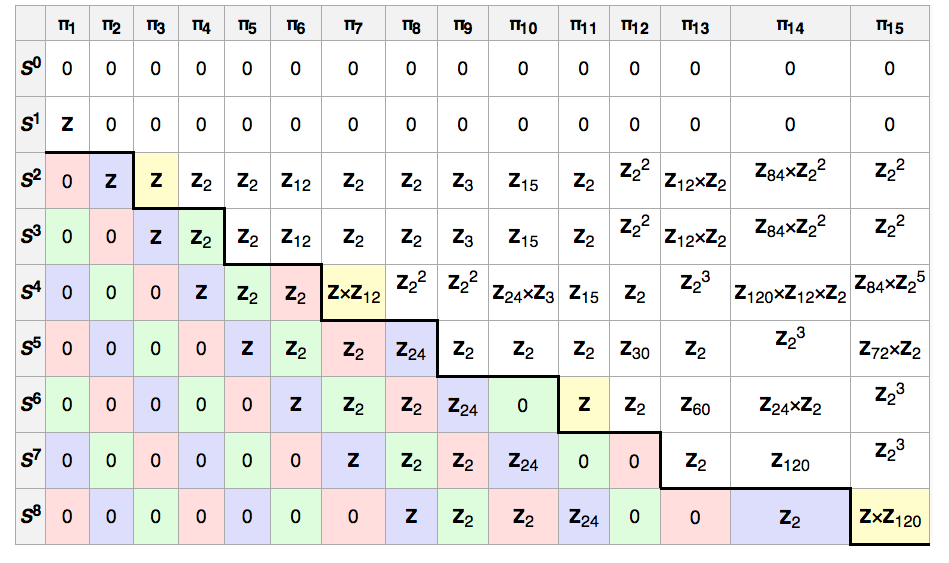
\includegraphics[width=5.5in]{spheres.png}

There are some patterns, but there is no general formula, and many
homotopy groups of spheres are currently unknown.  Homotopy groups are
just one of the algebraic invariants that people study; some others are
the \emph{homology groups} and \emph{cohomology groups}, which are
sometimes easier to calculate.

An interesting fact is that, while we started off by trying to classify
spaces up to isomorphism, most of these algebraic tools classify
spaces up to something called \emph{homotopy equivalence}.  Two spaces $X$ and $Y$
are called {\em homotopy equivalent} if there are maps $f : X \rightarrow Y$ and $g : Y \rightarrow X$
such that there is a homotopy between $f \circ g$ and the identity function on $Y$,
and similarly for $g \circ f$.  This gives you a little wiggle room to
``correct'' maps that don't exactly compose to the identity.
Isomorphic spaces are homotopy
equivalent, but not vice versa: for example, the disk is not isomorphic
to the point, but it is homotopy equivalent to it.  The vast majority of
the constructions one considers (homotopy groups, homology and
cohomology groups, etc.) are homotopy invariant, in the sense that they
respect homotopy equivalence.  For example, two homotopy equivalent
spaces have the same fundamental groups, essentially because the
fundamental group was defined to be paths modulo homotopy.  Thus, these
invariants are really properties of the homotopy equivalence classes of
spaces, which are called \emph{homotopy types}.  Homotopy equivalence is a coarser
relation on spaces that homeomorphism, so it can bear 
                                                         on the original
problem of classifying spaces up to homeomorphism, in that two spaces
that are shown to be not homotopy equivalent are then not homeomorphic.

\subsection{Homotopy theory of $\infty$-groupoids}

A natural setting for studying homotopy theory is $\infty$-groupoids, because
the formalism allows only notions invariant under homotopy to be formulated.
The notions of the previous section are all invariant under homotopy.
                                       Recall from Chapter~\ref{FIXME}
that $\infty$-groupoids are an infinite-dimensional generalization of
the categorical notion of a groupoid (which is a category where every
morphism is invertible).  Where a groupoid has just objects and
morphisms, $\infty$-groupoids have objects, morphisms, morphisms between
morphisms (2-morphisms), \dots, all the way up.  The structure of an $\infty$-groupoid is
complex: morphisms at each level have identity, composition,
and inverse operations, which are weak in the sense that they satisfy
the groupoid laws (associativity of composition, identity is a unit for
composition, inverses cancel) only up to morphisms at the next level.
Because of weakness, it is difficult to describe all the
operations on morphisms and all the properties of morphisms.  For example, because associativity
of composition of morphisms $p \ct (q \ct r) = (p \ct q) \ct r$ is
itself a higher-dimensional morphism, one needs an additional operation
relating various proofs of associativity: the various
ways to reassociate $p \ct (q \ct (r \ct s))$ into $((p \ct q) \ct r)
\ct s$ give rise to Mac Lane's pentagon.  Weakness also creates
non-trivial interactions between levels, such as the middle-four
interchange law.

Every topological space X has a fundamental $\infty$-groupoid whose
$k$-morphisms are the $k$-dimensional paths in $X$.  The weakness of the
$\infty$-groupoid (the fact that the groupoid laws hold only up to
higher-dimensional morphisms) corresponds directly to the fact that
paths form a group only up to homotopy, with the $k+1$-paths serving as the
homotopies between the $k$-paths.  Moreover, the view of a space as an
$\infty$-groupoid preserves enough structure to do homotopy theory
(calculate homotopy/homology/cohomology groups, etc.)  Formally, the
fundamental $\infty$-groupoid construction is adjoint to the geometric
realization of an $\infty$-groupoid as a space, and this adjunction
preserves homotopy theory (this is called the \emph{homotopy
  hypothesis/theorem}, because whether it is a hypothesis or theorem
depends on how you define $\infty$-groupoid).  For example, you can
easily define the fundamental group of an $\infty$-groupoid, and if you
calculate the fundamental group of the fundamental $\infty$-groupoid of
a space, and it will agree with the classical definition of fundamental
group.  So homotopy theory done in the setting of $\infty$-groupoids
really does tell you something about the original topological spaces
that you start with.  

\subsection{Homotopy theory in type theory}

Type theory is a formal calculus of $\infty$-groupoids. Because you can
do homotopy theory through the abstraction of $\infty$-groupoids, you
can do homotopy theory in type theory.  One might call this
\emph{synthetic homotopy theory}, by analogy with \emph{synthetic
  geometry}, which is geometry in the style of Euclid: you start from
some basic constructions (a line connecting any two points) and axioms
(all right angles are equal), and deduce consequences from them
logically.  Here, the basic constructions/axioms are the operations on
$\infty$-groupoids and maps between them ($\infty$-functors).  The
really nice thing about using HoTT to work with $\infty$-groupoids is
that you don't start by defining "an $\infty$-groupoid is..." like one
would in any other framework---which is fortunate, because describing
the structure of an $\infty$-groupoid in something like set theory is
notoriously difficult.  Instead, you exploit the fact that every type in
type theory is an $\infty$-groupoid, with the structure of morphisms,
2-morphism, 3-morphisms, ... given by the identity type.  We will often
refer to features of type theory by topological-sounding names (for
example, thinking of $p : \id[A] M N$ as a ``path'' from $M$ to $N$),
but it's important to keep in mind that we can only talk about these
things through the abstraction of an $\infty$-groupoid.

There are few really nice advantages of doing synthetic homotopy theory
in type theory.  First, you can use proof assistants like Agda and Coq
to check your proofs.  Second, we're starting to see examples where
working in type theory is suggesting new ways of doing proofs.  Third,
it seems likely that we will be able to interpret type theory in a wide
variety of other categories that ``look like'' the category of
$\infty$-groupoids ($(\infty,1)$-toposes), and, if so, proving a result
in type theory will show that it holds in these settings as well. It
remains to be seen how much homotopy theory we can do synthetically, but
there are already some positive indication, which are listed below.

The main tools we use to do homotopy theory in type theory are:

\subsubsection{Higher inductive types} To do some homotopy theory, we need some
  basic spaces (the circle, the sphere, the torus) and constructions for
  making new spaces (suspensions, gluing on cells, ...).  These are
  defined using higher inductive types, as described in
  \autoref{cha:hits}.

\subsubsection{Homotopy groups}  Having defined some spaces, we can start
  calculating some algebraic invariants of them.  The homotopy groups
  have an extremely natural definition in the setting of
  $\infty$-groupoids, which we import easily into type theory.  The fundamental group of $X$ at $x_0$
  is (to a first approximation---see below) just the identity type
  $\id[X] {x_0} {x_0}$, or the morphisms of the $\infty$-groupoid;
  $\pi_2(X,x_0$) is just the identity type $\id[{\id[X] {x_0} {x_0}}]
  {\refl{}}{\refl{}}$ the 2-morphisms, and so on.  So, calculating a
  homotopy group is just giving an equivalence between an identity type
  and some other type, and proving that this equivalence preserves the
  group structure.  For example, calculating the fundamental group of
  the circle consists of giving a equivalence between $\id[{\Sn ^1}]
  \base \base$ and $\Z$ that sends composition of paths to
  addition.

The reason this problem is interesting is that the (higher) inductive
definition of a type X presents X as a free $\infty$-groupoid, and this
presentation \emph{determines} but does not \emph{explicitly describe}
the higher identity types of X.  The identity types are populated by
both the generators ($\lloop$, for the circle), and all of the groupoid
operations (identity, composition, inverses, ...).  As the above table
for spheres shows, in higher dimensions the $\infty$-groupoid operations
create quite a complex structure.  Thus, the higher-inductive
presentation of a space allows you to pose the question "what does the
identity type of $X$ really turn out to be?", though it can take some
significant math to answer it.  This is a higher-dimensional
generalization of a familiar fact in type theory: even for ordinary
inductive types like natural numbers or booleans, it takes a bit of work
to prove that $\mathsf{true}$ is different from $\mathsf{false}$---characterizing the
identity type on booleans is a theorem, not part of the definition
(see \autoref{sec:compute-coprod}).

One detail that was glossed over above is that the (iterated) identity
type really gives what is called the \emph{path space} of a space, which
is not just the \emph{set} of $k$-dimensional paths, but a whole space
of them, with their higher homotopies.  To extract the set of
paths-modulo-homotopy, we can use truncation, as described in
\autoref{cha:hits}.  For example, the fundamental group of a
space is defined to be the 0-truncation of the space of loops at $x_0$,
which produces the set of paths modulo homotopy, killing the higher
homotopies of the loop space.

Using iterated loop spaces (\cref{def:loopspace}), we can make the
following definition:
\begin{defn}
  Given $n:\N$ and $(A,a)$ a pointed type, we define the homotopy groups of $A$
  at $a$ by
  \[\pi_n(A,a)=\trunc0{\Omega^n(A,a)}\]
\end{defn}

\subsubsection{Univalence}  The univalence axiom plays an essential role in
  calculating homotopy groups (this is a formal claim: without
  univalence, type theory is compatible with an interpretation where all
  paths, including, for example, the loop on the circle, are reflexivity).  You
  can see this in the calculation of the the fundamental group of the
  circle below: the map from $\id[\Sn ^1] \base \base$ to $\Z$
  is defined by mapping a path on the circle to an isomorphism on
  $\Z$, so that, for example, $\lloop \ct \opp \lloop$ is sent
  to $successor \ct predecessor$, and then applying the isomorphism to
  0. Univalence allows non-trivial paths in the universe, and this is
  used to extract information from paths in higher inductive types.

\subsubsection{Homotopy-theoretic and type-theoretic methods}  In the
proofs we've done so far, we've found that there are various ways of
doing homotopy theory in HoTT.  Some proofs use techniques that are
familiar from traditional homotopy theory and category theory, such as
contractibility of total spaces of fibrations, or properties of
pushout/pullback diagrams.  Others are more type-theoretic, and consist
mainly of calculations with the $\infty$-groupoid structure, in a style
that is very similar to how computer-scientists use type theory to
reason about programs.  The line between the two styles is fuzzy, and
many proofs have aspects of both styles; but there is enough of a
difference in ``feel'' that it is worth commenting on.  We will present
some examples of both styles below, and describe an example of the
difference in \autoref{sec:pi1-s1-intro}.

\subsection{Theorems we have proved}

Here is a sample of some high-level theorems that we have proved in
HoTT.  These are all well-known results in algebraic topology; the
interesting thing is that they can be carried out in HoTT, and, in most
cases, they have been computer-checked.

\begin{thm}[Homotopy Groups of Spheres] \mbox{}
\begin{itemize}
\item $\pi_n(\Sn ^n) = \Z$ for $n \ge 1$.
\item $\pi_k(\Sn ^n) = 1$ for $k < n$.  
\item $\pi_3(\Sn ^2) = \Z$
\item $\pi_{n+1}(\Sn ^n) = \Z_2$ for $n \ge 3$.    
\item $\pi_k(\Sn ^n) = \pi_{k+1}(\Sn ^{n+1})$ whenever $k \le 2n - 2$.  
\end{itemize}
\end{thm}

\begin{thm}[Hopf Fibration]
There is a fibration $H$ over $\Sn ^2$ whose fibers are $\Sn ^1$ and
whose total space is $\Sn ^3$.  
\end{thm}

\begin{thm}
  If $X$ is $n$-connected, then $\pi_k(X) = 1$ for $k < n$.
\end{thm}

Recall from \autoref{sec:suspension} that $\susp X$ denotes the suspension of $X$.

\begin{thm}[Freudenthal Suspension Theorem]
  If $X$ is $n$-connected, the map $X \rightarrow \Omega(\susp X)$ is $2n$-connected.
  In particular, $\id{\trunc{2n}{X}}{\trunc{2n}{\Omega(\susp X)}}$.
\end{thm}

Recall from \autoref{sec:colimits} that $X \sqcup^C Y$ is the pushout of $X$ and $Y$ along $C$.

\begin{thm}[Blakers-Massey Theorem]
  If $X$ is $i$-connected and $Y$ is
  $j$-connected, then for all $x:X$ and $y:Y$, the map $\glue : C(x,y)
  \rightarrow X \sqcup^C Y$ is $i+j$-connected.  In
  particular, $\trunc {i+j} {P(x,y)} = \trunc {i+j} {\id [X \sqcup^C Y]
    {(\inl(x))} {(\inr(y))}}$.\note{What is $P$?}
\end{thm}

\begin{thm}[Eilenberg--Mac Lane Spaces]
For any abelian group $G$ and positive number $n$, there is a type
$K(G,n)$ such that $\pi_n(K(G,n)) = G$, and  $\pi_k(K(G,n)) = 1$
for $k\neq n$.
\end{thm}

\begin{thm}[Van Kampen Theorem]
For any maps $f:A\to B$ and $g:A\to C$ with $A$ connected, the fundamental group of the homotopy pushout of $f$ and $g$ is the amalgamated free product (pushout of groups) of $\pi_1(B)$ and $\pi_1(C)$ over $\pi_1(A)$:
\[ \pi_1(B\sqcup_A C) = \pi_1(B) *_{\pi_1(A)} \pi_1(C).\]
There is also a generalization to non-connected $A$.
\end{thm}

\begin{thm}[Whitehead's Principle for $n$-types]
If $X$ and $Y$ are $n$-types, and $f : X \rightarrow Y$ induces an
isomorphism $\id{\pi_k(X)}{\pi_k(Y)}$ for all $k \le n$, then $f$ is an
equivalence.
\end{thm}

As discussed above, some proofs have a more homotopy-theoretic style,
while others have a more type-theoretic style.  Many theorems can be
proved in both styles.  The type-theoretic proofs are generally easier
to formalize as computer-checked proofs.  In part, this is because the
homotopy-theoretic proofs often prove a stronger lemma than is strictly
necessary, but which may be of independent interest: For example, for
$\pi_2(\Sn ^2)$, the homotopy-theoretic proof requires proving that the
total space of the Hopf fibration (represented as a dependent type) is
$\Sn ^3$, a significant result in its own right, whereas the
type-theoretic proof bypasses this result, replacing it with
calculations using the definition of the Hopf fibration.  It is
currently unclear whether the type-theoretic style can be used to prove
some of the most difficult theorems, such as the total space of Hopf
fibration and $\pi_3(\Sn ^2)$ and $\pi_4(\Sn ^3)$, which we have done in
the homotopy-theoretic style.

\autoref{tab:theorems} lists the proofs we have done in each style, and
whether they have been computer-checked (\checkmark) or only done
informally.  For the spheres, we have used two different definitions of
the $n$-sphere $\Sn ^n$: the first as the suspension of $\Sn ^ {n-1}$,
and the second as a higher inductive type with one base point and one
loop in $\Omega^n$; we list the status for both definitions.

\begin{table}
  \centering
\begin{tabular}{l|l|l}
Theorem         & Homotopy-theoretic style & Type-theoretic style\\
\hline 
$\pi_1(\Sn ^1)$ & \checkmark & \checkmark \\ 
\hline 
$\pi_{k<n}(\Sn ^n)$ --- single-loop &    & \checkmark \\
$\pi_{k<n}(\Sn ^n)$ --- suspension  &  \checkmark?  & \checkmark \\
\hline 
$\pi_2(\Sn ^2)$ --- single-loop &   &  \checkmark \\
$\pi_2(\Sn ^2)$ --- suspension & informal   & \checkmark \\
\hline 
total space of Hopf fibration & informal &  \\
\hline 
$\pi_3(\Sn ^2)$     & informal   & \\
\hline 
$\pi_n(\Sn ^n)$ --- single-loop &    & \checkmark \\
$\pi_n(\Sn ^n)$ --- suspension  &  informal  & \checkmark \\
\hline 
$\pi_4(\Sn ^3)$  &  informal  &  \\
\hline
Freudenthal         &  informal  & \checkmark \\
\hline 
Blakers-Massey      &            & informal  \\
\hline 
$K(G,n)$              &            & \checkmark  \\
\hline 
naive Van Kampen              &            & \checkmark  \\
\hline
improved Van Kampen              &            & informal \\
\hline
Whitehead for $n$-types  &  &  \checkmark 
\end{tabular}
  \caption{Theorems from homotopy theory}
  \label{tab:theorems}
\end{table}


\section{Some basic homotopy groups}

In this section, we describe some basic examples of calculating homotopy
groups, which can be carried out using the tools we have developed so
far.  Unless otherwise stated, the notation \type will denote a
\emph{fixed} universe and several occurrences of the word \type will
always represent the same universe. The types \prop, \set, \typele{n}
represent the types of propositions, sets and $n$-truncated types of
this fixed universe \type.

\subsection{\texorpdfstring{$\pi_1(S^1)$}{π₁(S¹)}}
\label{sec:pi1-s1-intro}

Our goal is to show that $\id {\pi_1(\Sn ^1)} {\Z}$.  In fact, we
will show that the loop space $\id {\Omega(\Sn ^1)} {\Z}$.  This is a stronger
statement, because $\id{\pi_1(\Sn ^1)} {\trunc 0 {\Omega(\Sn ^1)}}$ by
definition, so if $\id {\Omega(\Sn ^1)} {\Z}$, then $\id {\trunc
  0 {\Omega(\Sn ^1)}} {\trunc 0 {\Z}}$ by congruence, and
$\Z$ is a set, so $\id {\trunc 0 {\Z}} {\Z}$
(FIXME: do we have this somewhere?).  
\note{What definition of $\Z$ do we want to use?}

Our proof that $\Omega_1(\Sn ^1)$ is $\Z$ can be seen as a
type-theoretic version of a proof in classical homotopy theory.  The
classical proof we start from is usually formulated using ``universal
covering spaces'', but we will give an equivalent sketch using
\emph{fibrations} which transfers more directly to type theory.  For any
point $x_0\in B$, there is a canonical \emph{path fibration} $p:P_{x_0}
B \to B$, where the points of $P_{x_0} B$ are paths in $B$ starting at
$x_0$, and the map $p$ selects the other endpoint of such a path.  The
space $P_{x_0} B$ is \emph{contractible}, i.e., homotopy equivalent to a
point, since we can ``retract'' any path to its initial endpoint $x_0$.
Moreover, the fiber over $x_0$ is the loop space $\Omega_1(B,x_0)$.

Now consider the ``winding'' map $w:\mathbb{R}\to \Sn ^1$, which
looks like a helix projecting down onto the circle:
\begin{center}
  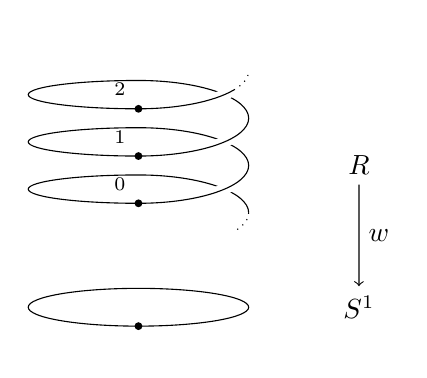
\begin{tikzpicture}[xscale=1.4,yscale=.6]
    \node (R) at (2,1) {$\mathbb{R}$};
    \node (S1) at (2,-2) {$S^1$};
    \draw[->] (R) -- node[auto] {$w$} (S1);
    \draw (0,-2) ellipse (1 and .4);
    \draw[dotted] (1,0) arc (0:-30:1 and .8);
    \draw (1,0) arc (0:90:1 and .8) arc (90:270:1 and .3) coordinate (t1);
    \draw[white,line width=4pt] (t1) arc (-90:90:1 and .8);
    \draw (t1) arc (-90:90:1 and .8) arc (90:270:1 and .3) coordinate (t2);
    \draw[white,line width=4pt] (t2) arc (-90:90:1 and .8);
    \draw (t2) arc (-90:90:1 and .8) arc (90:270:1 and .3) coordinate (t3);
    \draw[white,line width=4pt] (t3) arc (-90:90:1 and .8);
    \draw (t3) arc (-90:-30:1 and .8) coordinate (t4);
    \draw[dotted] (t4) arc (-30:0:1 and .8);
    \node[fill,circle,inner sep=1pt,label={below:\scriptsize \base}] at (0,-2.4) {};
    \node[fill,circle,inner sep=1pt,label={above left:\scriptsize 0}] at (0,.2) {};
    \node[fill,circle,inner sep=1pt,label={above left:\scriptsize 1}] at (0,1.2) {};
    \node[fill,circle,inner sep=1pt,label={above left:\scriptsize 2}] at (0,2.2) {};
  \end{tikzpicture}
\end{center}
The map $w$ sends each point on the helix to the point on the circle
that it is ``sitting above''; this map is a fibration, and the fiber
over each point is isomorphic to the integers.  If we lift the path that
goes counterclockwise around the loop on the bottom, we go up one level in the
helix, incrementing the integer in the fiber.  Similarly, going
clockwise around the loop on the bottom corresponds to going down
one level in the helix, decrementing this count.  This fibration is
called the \emph{universal cover} of the circle.

Now a basic fact is that a map $E_1\to E_2$ of fibrations over $B$
which is a homotopy equivalence between $E_1$ and $E_2$ induces a
homotopy equivalence on fibers.  Since $\mathbb{R}$ and $P_{\base} S^1$
are both contractible, they are homotopy equivalent, and thus the fibers
over \base, $\Z$ and $\Omega_1(\Sn ^1)$, are isomorphic.

\smallskip

It is possible to directly formalize this classical homotopy-theoretic
proof in type theory, by (1) defining the universal cover, (2) proving
that a homotopy equivalence between total spaces induces an equivalence
on fibers, and (3) proving that the total spaces of both the path
fibration and the cover are contractible. Indeed, this was the first
proof of this result in HoTT.

We later discovered that there is an alternative proof, which has a more
type-theoretic feel.  In this proof, you directly construct fiberwise
maps between the path fibration and the universal cover, and prove that
they are mutually inverse by calculation.  We will call this the
\emph{type-theoretic} or \emph{encode/decode} proof, because
\emph{encode} and \emph{decode} are the names we use for the fiberwise
maps between the path fibration and the cover below.  Both proofs use
the same construction of the cover (step 1 above).  Where the classical
proof induces an equivalence on fibers from an equivalence between total
spaces (step 2), the encode/decode proof constructs the inverse map
(\emph{decode}) explicitly as a map between fibers.  Where the classical
proof uses contractibility (step 3), the type-theoretic proof uses path
induction, circle induction, and integer induction.  These are the same
tools used to prove contractibility---indeed, path induction \emph{is}
contractibility of the path fibration composed with
$\mathsf{transport}$, but they are applied in a different way.

\subsubsection{Encode/decode proof}

By definition, $\Omega(\Sn ^1)$ is $\id[\Sn ^1] \base \base$.  If we
attempt to prove that $\id {\Omega(\Sn ^1)} {\Z}$ by directly
constructing an equivalence, we will get stuck, because type theory
gives you little leverage for working with loops.  Instead, we
generalize the theorem statement to the path fibration, and analyze the
whole fibration
\[
P(x:\Sn ^1) \defeq (\id[\Sn ^1] \base x)
\]
with one end-point free.  

We show that $P(x)$ is equal to another fibration, which gives a more
explicit description of the paths---we call this other fibration
``codes'', because its elements are \emph{data} that act as codes for
paths on the circle.  In this case, the codes fibration is the universal
cover of the circle.

\begin{defn}[Universal Cover of $\Sn ^1$]
Define $\code(x:\Sn ^1) : \type$ by circle-recursion, with 
\[
\begin{array}{l}
\code(\base) \defeq \Z \\
\ap{\code}{\lloop} \defeq \ua(\Zsuc) \\
\end{array}
\]
where $\Zsuc$ is the equivalence $\eqv {\Z} {\Z}$ given by
adding one, which by univalence determines a path from $\Z$ to
$\Z$ in \type.  
\end{defn}

To define a function by circle recursion, we need to find a point and a
loop in the target.  In this case, the target is $\type$, and the point
we choose is $\Z$, corresponding to our expectation that the
fiber of the universal cover should be the integers.  The loop we choose
is the successor/predecessor isomorphism on $\Z$, which
corresponds to the fact that going around the loop in the base goes up
one level on the helix.  Univalence is necessary for this part of the
proof, because we need a \emph{non-trivial} equivalence on $\Z$.  

From this definition, it is simple to calculate that transporting with
$\code$ takes $\lloop$ to the successor function, and 
$\opp{\lloop}$ to the predecessor function:
\begin{lem} \label{lem:transport-s1-code}
\id{\transfib \code \lloop x} {x + 1} and 
\id{\transfib \code {\opp \lloop} x} {x - 1}
\end{lem}
\begin{proof}
For the first, we calculate as follows:
\[
\begin{array}{lll}
 & {\transfib \code \lloop x} &\\
= & \transfib {A \mapsto A} {(\ap{\code}{\lloop})} x & \text{associativity}\\
= & \transfib {A \mapsto A} {\ua (\Zsuc)} x & \text{reduction for circle-recursion}\\
= & x + 1 & \text{reduction for \ua}
\end{array}
\]
The second follows from the first, because 
$\transfibf B p$ and 
and ${\transfibf B {\opp p}}$ are always inverses, so 
$\id{\transfibf \code {\opp \lloop}}$ must be the inverse of the
$- + 1$.  
\end{proof}

In the remainder of the proof, we will show that $P$ and $\code$ are
equivalent.  

\paragraph{Encoding}

Next, we define a function \encode that maps paths to codes:
\begin{defn}
Define $\encode : \prd{x : \Sn ^1} \rightarrow P(x) \rightarrow  \code(x)$ by 
\[
\encode \: p \defeq \transfib{\code} p 0
\]
(we leave the argument $x$ implicit).  
\end{defn}
Encode is defined by lifting a path into the universal cover, which
determines an equivalence, and then applying the resulting equivalence
to $0$.  
The interesting thing about this function is that it computes a concrete
number from a loop on the circle, when this loop is represented using
the abstract groupoidal framework of HoTT.  To gain an
intuition for how it does this, observe that by the above lemmas,
$\transfib \code \lloop x$ is $-+1$ and $\transfibf \code {\opp
  \lloop} x$ is $x - 1$.  Further, $\mathsf{transport}$ is functorial
(\autoref{cha:basics}), so $\transfibf{\code} {\lloop \ct \lloop}$ is
$(\transfibf \code \lloop) \circ (\transfib \code \lloop)$, etc.  Thus, when $p$ is a
composition like 
\[
\lloop \ct \opp \lloop \ct \lloop \ct ...
\]
$\transfibf{\code}{p}$ will compute a composition of functions like
\[
(- + 1) \circ (- -1) \circ (- + 1) \circ ... 
\]
Applying this composition of functions to 0 will compute the
\emph{winding number} of the path---how many times it goes around the
circle, with orientation marked by whether it is positive or negative,
after inverses have been canceled.  Thus, the computational behavior of
$\encode$ follows from the reduction rules for higher-inductive types and
univalence, and the action of $\mathsf{transport}$ on compositions and inverses.

Note that the instance $\encode' \defeq \encode_{\base}$ has type 
$\id \base \base \rightarrow \Z$, which will be one half of the
equivalence between $\id{\base}{\base}$ and $\Z$.  

\paragraph{Decoding}  

Decoding an integer as a path is defined by recursion:

\begin{defn}
Define $\lloop^- : \Z \rightarrow \id{\base}{\base}$ by 
\[
\lloop^n = \begin{cases} \lloop \ct \lloop \ct ... \ct \lloop \text{ ($n$ times) } & \text{for positive n} \\
 \opp \lloop \ct \opp \lloop \ct ... \ct \opp \lloop \text{ ($n$ times)} & \text{for negative n} \\
  \refl{} & \text{for 0}  
\end{cases}
\]
\end{defn}

Since what we want overall is an equivalence between $\id \base \base$
and $\Z$, we might expect to be able to prove that $\encode'$
and $\lloop^-$ give an equivalence.  The problem comes in trying to prove
the ``decode after encode'' direction, where we would need to show that
$\id {\lloop^{\encode' p}} p$ for all $p$.  We would like to apply path
induction, but path induction does not apply to loops like a with both
endpoints fixed!  The way to solve this problem is to generalize the
theorem to show that $\id {\lloop^{{\encode_x p}}} p$ for all $x: \Sn ^1$
and $p : \id \base x$.  However, this does not make sense as is, because
$\lloop^-$ is defined only for \id{\base}{\base}, whereas here it is
applied to a \id{\base}{x}.  Thus, we generalize 
$\lloop$ as follows:

%% deliberately making a ``definition'' with a proof here :-) --Dan
\begin{defn}
Define $\decode : \prd{x : \Sn ^1}{\code(x) \rightarrow P(x)}$ by 
circle induction on $x$.  It suffices to give a function 
${\code(\base) \rightarrow P(\base)}$, for which we use $\lloop^-$, and 
to show that $\lloop^-$ respects the loop.  
\end{defn}

\begin{proof}
To show that $\lloop^-$ respects the loop, it suffices to give a path
from $\lloop^-$ to itself that lies over $\lloop$. 
Formally, this means a path from $\transfib {(x' \mapsto Cover x'
\rightarrow P(x'))} {\lloop} {\lloop^-}$ to $loop^-$.  We define such a
path as follows:

\[
\begin{array}{lll}
  & \transfib {(x' \mapsto \code(x') \rightarrow P(x'))} \lloop {\lloop^-} & \\
= & \transfibf P \lloop \circ {\lloop^-} \circ \transfibf \code {\opp \lloop} & \\
= & (- \ct \lloop) \circ (\lloop^-) \circ \transfibf \code {\opp \lloop} & \\
= & (- \ct \lloop) \circ (\lloop^-) \circ (- - 1) & \\
= & (n \mapsto \lloop^{n - 1} \ct \lloop) \\                       
\end{array}
\]

From line 1 to line 2, we apply the definition of $\mathsf{transport}$
when the outer connective of the fibration is $\rightarrow$, whcih
reduces the $\mathsf{transport}$ to pre- and post-composition with
$\mathsf{transport}$ at the domain and range types.  From line 2 to line
3, we apply the definition of $\mathsf{transport}$ when the type family
is $\id{\base}{x}$, which is post-composition of paths.  From line 3 to
line 4, we use the action of $\code$ on $\opp \lloop$ defined in
\autoref{lem:transport-s1-code}.  From line 4 to line 5, we simply
reduce the function composition.  Thus, it suffices to show that for all
$n$, \id{\lloop^{n - 1} \ct \lloop}{\lloop^{n}}, which is an easy
induction, using the groupoid laws.  
\end{proof}

\paragraph{Decoding after encoding}

\begin{lem} \label{lem:s1-decode-encode}  For all 
for all $x: \Sn ^1$ and $p : \id \base x$, $\id
{\decode_x({{\encode_x(p)}})} p$.  
\end{lem}

\begin{proof}
By path induction, it suffices to show that 
$\id {\decode_{\base}({{\encode_{\base}(\refl{\base})}})} {\refl{\base}}$.  But
${\encode_{\base}(\refl{\base})} \jdeq 
 \transfib{\code}{\refl{\base}} 0 \jdeq 0$, and $\decode_{\base}(0)
 \jdeq \lloop^ 0 \jdeq \refl{\base}$.  
\end{proof}

\paragraph{Encoding after decoding}

\begin{lem} \label{lem:s1-encode-decode} For all 
for all $x: \Sn ^1$ and $c : \code(x)$, $\id
{\encode_x({{\decode_x(c)}})} c$.  
\end{lem}

\begin{proof}
The proof is by circle induction.  It suffices to show the case for
\base, because the case for \lloop is a path between paths in
$\Z$, which can be given by appealing to the fact that $\Z$ is a set.  

Thus, it suffices to show, for all $n : \Z$, that
\[
\id {\encode'(\lloop^n)} {n}
\]
The proof is by induction, with cases for $0$,$1$,$-1$,$n+1$, and
$n-1$.  

\begin{itemize}

\item In the case for $0$, the result is true by definition.

\item In the case for $1$, ${\encode'(\lloop^1)}$ reduces to 
$\transfib{\code}{\lloop}{0}$, which by
\autoref{lem:transport-s1-code} is $0 + 1 = 1$.  

\item In the case for $n+1$, 
\[
\begin{array}{lll}
  & {\encode'(\lloop^{n+1})}  \\
= & {\encode'(\lloop^{n} \ct \lloop)} & \\
= & \transfib{\code}{(\lloop^{n} \ct \lloop)}{0} & \\
= & \transfib{\code}{\lloop}{(\transfib{\code}{(\lloop^n)}{0})} & \text{by functoriality}\\
= & {(\transfib{\code}{(\lloop^n)}{0})} + 1 & \text{by \autoref{lem:transport-s1-code}}\\
= & n + 1 & \text{by the IH} \\
\end{array}
\]

\item The cases for negatives are analogous.  
\end{itemize}
\end{proof}

\paragraph{Tying it all togehter}

\begin{thm}
There is a family of equivalences $\prd{x : \Sn ^1} {\eqv {P(x)} {\code(x)}}$.  
\end{thm}
\begin{proof}
The maps $\encode$ and $\decode$ are mutually inverse by 
\autoref{lem:s1-decode-encode,lem:s1-decode-encode},
and this can be improved to an equivalence.  
\end{proof}

Instantiating at {\base} gives
\begin{cor}\label{cor:omega-s1}
$\eqv {(\id{\base}{\base})} {\Z}$
\end{cor}

A simple induction shows that this equivalence takes addition to
compostion, so $\Omega(\Sn ^1) = \Z$ as groups.  

\begin{cor}
$\id{\pi_k(\Sn ^1)} {\Z}$ if $k = 1$ and $1$ otherwise.  
\end{cor}
\begin{proof}
For $k=1$, we sketched the proof from \autoref{cor:omega-s1} above.
For $k > 1$, $\trunc 0 {\Omega^{n+1}(\Sn ^1)} = \trunc 0
{\Omega^n(\Omega{\Sn ^1})} = \trunc 0 {\Omega^n(\Z)}$, which is
  $1$ because $\Z$ is a set and $\pi_n$ of a set is trivial (FIXME
  lemmas to cite?).
\end{proof}


\subsection{Van Kampen's theorem}
\label{sec:van-kampen}

Van Kampen's theorem calculates the fundamental group $\pi_1$ of a pushout of spaces.
It is traditionally stated for a topological space $X$ which is the union of two open subspaces $U$ and $V$, but in homotopy-theoretic terms this is just a convenient way of ensuring that $X$ is the homotopy pushout of $U$ and $V$ over their intersection.
Thus, we will prove a version of van Kampen's theorem for arbitrary homotopy pushouts.

In this section we will describe a proof of van Kampen's theorem which uses the same type-theoretic encode/decode machinery that we used for $\pi_1(\Sn^1)$ in \autoref{sec:pi1-s1-intro}.
There is another more homotopy-theoretic approach, which uses the machinery of reflective subuniverses to be described in \autoref{sec:more-advanced-tools}.

We do need a more refined version of the encode/decode technique, however.
In \autoref{sec:pi1-s1-intro} (as well as in \autoref{sec:compute-coprod,sec:compute-nat}) we used it to characterize the entire path spaces of a (higher) inductive type $W$ --- deriving as a consequence a characterization of the loop space $\Omega(W)$, and thereby also of its 0-truncation $\pi_1(W)$.
In van Kampen's theorem, our goal is only to characterize the fundamental group $\pi_1(W)$, and we do not have any explicit description of the loop spaces or the path spaces to use.
However, it turns out that we can use the same technique directly for a truncated version of the path spaces, thereby characterizing not only the fundamental \emph{group} $\pi_1(W)$ but the whole 0-truncated path fibration.


\subsubsection{Naive van Kampen}
\label{sec:naive-vankampen}

We begin with a ``naive'' version of van Kampen's theorem, which is useful but not quite as useful as the classical version.
In \autoref{sec:better-vankampen} we will improve it to a more useful version.

For a type $X$, write $\Pi_1 X: X\to X\to \type$ be the $0$-truncation of its identity type, i.e., $\Pi_1 X(x,y) \defeq \trunc0{x=y}$.
Note that we have induced groupoid operations
\begin{gather*}
  (-\ct-) : \Pi_1X(x,y) \to \Pi_1X(y,z) \to \Pi_1X(x,z)\\
  \opp{(-)} : \Pi_1X(x,y) \to \Pi_1X(y,x)\\
  \refl{x} : \Pi_1X(x,x)\\
  \apfunc{f} : \Pi_1X(x,y) \to \Pi_1Y(fx,fy)
\end{gather*}
for which we use the same notation as the corresponding operations on paths.

Now given types $A,B,C$ and functions $f:A\to B$ and $g:A\to C$, let $P$ be the higher inductive type generated by
\begin{itemize}
\item $i:B\to P$
\item $j:C\to P$
\item for all $x:A$, a path $k x:ifx = jgx$.
\end{itemize}
Define $\code:P\to P\to \type$ by double induction on $P$ as follows.
\begin{itemize}
\item $\code(ib,ib')$ is a set-quotient of the type of sequences %pairs $(\vec a, \vec a', \vec p, \vec q)$
  \[ (b, p_0, x_1, q_1, y_1, p_1, x_2, q_2, y_2, p_2, \dots, y_n, p_n, b') \]
  where
  \begin{itemize}
  \item $n:\mathbb{N}$
  \item $x_k:A$ and $y_k:A$ for $0<k \le n$
  \item $p_0:\Pi_1B(b,f x_1)$ and $p_n:\Pi_1B(f y_n, b')$
  \item $p_k:\Pi_1B(f y_k, fx_{k+1})$ for $1\le p < n$
  \item $q_k:\Pi_1C(gx_k, gy_k)$ for $1\le q\le n$
  \end{itemize}
  The quotient is generated by the following equalities:
  \begin{alignat*}{2}
    % (\dots, p_{k-1} \ct fw, x_{k}', q_{k}, \dots) &=
    % (\dots, p_{k-1}, x_{k}, gw \ct q_{k}, \dots)
    % & \qquad\text{for } w:\Pi_1A(x_{k},x_{k}')\\
    % (\dots, q_k \ct gw, y_k', p_k, \dots) &=
    % (\dots, q_k, y_k, fw \ct p_k, \dots)
    % & \qquad\text{for } w:\Pi_1A(y_k, y_k')\\
    (\dots, q_k, y_k, \refl{fy_k}, y_k, q_{k+1},\dots)
    &= (\dots, q_k\ct q_{k+1},\dots)\\
    (\dots, p_k, x_k, \refl{gx_k}, x_k, p_{k+1},\dots)
    &= (\dots, p_k\ct p_{k+1},\dots)
  \end{alignat*}
  (see \autoref{rmk:naive} below).
\item $\code(jc,jc')$ is identical, with the roles of $B$ and $C$ reversed.
  We likewise notationally reverse the roles of $x$ and $y$, and of $p$ and $q$.
\item $\code(ib,jc)$ and $\code(jc,ib)$ are similar, with the parity changed so that they start in one type and end in the other.
\item For $a:A$ and $b:B$, we require an equivalence
  \begin{equation}
    \code(ib, ifa) \simeq \code(ib,jga).\label{eq:bfa-bga}
  \end{equation}
  We define this to consist of the two functions defined on sequences by
  \begin{align*}
    (\dots, y_n, p_n,fa) &\mapsto (\dots,y_n,p_n,a,\refl{ga},ga)\\
    (\dots, x_n, p_n, a, \refl{fa}, fa) &\mapsfrom (\dots, x_n, p_n, ga)
  \end{align*}
  Both of these functions are easily seen to respect the equivalence relations, and hence to define functions on the types of codes.
  The left-to-right-to-left composite is
  \[ (\dots, y_n, p_n,fa) \mapsto
  (\dots,y_n,p_n,a,\refl{ga},a,\refl{fa},fa)
  \]
  which is equal to the identity by a generating equality of the quotient.
  The other composite is analogous.
  Thus we have defined an equivalence~\eqref{eq:bfa-bga}.
\item Similarly, we require equivalences
  \begin{align*}
    \code(jc,ifa) &\simeq \code(jc,jga)\\
    \code(ifa,ib)&\simeq (jga,ib)\\
    \code(ifa,jc)&\simeq (jga,jc)
  \end{align*}
  all of which are defined in exactly the same way (the second two by adding reflexivity terms on the beginning rather than the end).
\item Finally, we need to know that for $a,a':A$, the following diagram commutes:
  \begin{equation}\label{eq:bfa-bga-comm}
  \vcenter{\xymatrix{
      \code(ifa,ifa') \ar[r]\ar[d] &
      \code(ifa,jga')\ar[d]\\
      \code(jga,ifa')\ar[r] &
      \code(jga,jga')
      }}
  \end{equation}
  This amounts to saying that if we add something to the beginning and then something to the end of a sequence, we might as well have done it in the other order.
\end{itemize}

\begin{rmk}\label{rmk:naive}
  You might expect to see in the definition of \code some additional generating equations for the set-quotient, such as
  \begin{alignat*}{2}
    (\dots, p_{k-1} \ct fw, x_{k}', q_{k}, \dots) &=
    (\dots, p_{k-1}, x_{k}, gw \ct q_{k}, \dots)
    & \qquad\text{for } w:\Pi_1A(x_{k},x_{k}')\\
    (\dots, q_k \ct gw, y_k', p_k, \dots) &=
    (\dots, q_k, y_k, fw \ct p_k, \dots)
    & \qquad\text{for } w:\Pi_1A(y_k, y_k').
  \end{alignat*}
  However, these are not necessary!
  In fact, they follow automatically by path-induction on $w$.
  This is because the requisite ``quotienting'' by paths in $A$ has happened already in the fact that $\code(u,v)$ is a \emph{set}, even though it involves the untruncated type $A$ in its definition.
  This is why the version of van Kampen we are currently describing is ``naive''.
  % In the next section we will remedy this defect.
\end{rmk}

Continuing on, we can characterize transporting in the fibration $\code$:
\begin{itemize}
\item For $p:b=_B b'$ and $u:P$, we have
  \[ \mathsf{transport}^{b\mapsto \code(u,ib)}(p, (\dots, y_n,p_n,b))
  = (\dots,y_n,p_n\ct p,b').
  \]
\item For $q:c=_C c'$ and $u:P$, we have
  \[ \mathsf{transport}^{c\mapsto \code(u,jc)}(q, (\dots, x_n,q_n,c))
  = (\dots,x_n,q_n\ct q,c').
  \]
\end{itemize}
Here we are abusing notation by using the same name for a path in $X$ and its image in $\Pi_1X$.
Note that transport in $\Pi_1X$ is also given by concatenation with (the image of) a path.
From this we can prove the above statements by induction on $u$.
We also have:
\begin{itemize}
\item For $a:A$ and $u:P$,
  \[ \mathsf{transport}^{v\mapsto \code(u,v)}(ha, (\dots, y_n,p_n,fa))
  = (\dots,y_n,p_n,a,\refl{ga},ga).
  \]
\end{itemize}
This follows essentially from the definition of $\code$.

We also construct a function
\[ r : \prod_{u:P} \code(u,u) \]
by induction on $u$ as follows:
\begin{align*}
  rib &\defeq (b,\refl{b},b)\\
  rjc &\defeq (c,\refl{c},c)
\end{align*}
and for $rka$ we take the composite equality
\begin{align*}
  (ka,ka)_* (fa,\refl{fa},fa)
  &= (ga,\refl{ga},a,\refl{fa},a,\refl{ga},ga) \\
  &= (ga,\refl{ga},ga)
\end{align*}
where the first equality is by the observation above about transporting in $\code$, and the second is an instance of the set quotient relation used to define $\code$.

We will now prove:
\begin{thm}[Naive van Kampen]
  For all $u,v:P$ there is an equivalence
  \[ \Pi_1P(u,v) \simeq \code(u,v). \]
\end{thm}
\begin{proof}

To define a function
\[ \encode : \Pi_1P(u,v) \to \code(u,v) \]
it suffices to define a function $(u=_P v) \to \code(u,v) $,
since $\code(u,v)$ is a set.
We do this by transport:
\[\encode(p) \defeq \mathsf{transport}^{v\mapsto \code(u,v)}(p,r(u)).\]
Now to define
\[ \decode: \code(u,v) \to \Pi_1P(u,v) \]
we proceed as usual by induction on $u,v:P$.
In each case for $u$ and $v$, we apply $i$ or $j$ to all the equalities $p_k$ and $q_k$ as appropriate and concatenate the results in $P$, using $h$ to identify the endpoints.
For instance, when $u\jdeq ib$ and $v\jdeq ib'$, we define
\begin{multline}\label{eq:decode}
 \decode(b, p_0, x_1, q_1, y_1, p_1, \dots, y_n, p_n, b')\\
 \defeq i(p_0)\ct h(x_1) \ct j(q_1) \ct \opp{h(y_1)} \ct i(p_1) \ct \cdots \ct \opp{h(y_n)}\ct i(p_n).
\end{multline}
This respects the set-quotient equivalence relation and the equivalences like~\eqref{eq:bfa-bga}, since $h: fi \sim gj$ is natural and $f$ and $g$ are functorial.

As usual, to show that the composite
\[ \Pi_1P(u,v) \xrightarrow{\encode} \code(u,v) \xrightarrow{\decode} \Pi_1P(u,v) \]
is the identity, we first peel off the 0-truncation (since the target is a set) and then apply path-induction.
The input $\refl{u}$ goes to $ru$, which then goes back to $\refl u$ (applying a further induction on $u$ to decompose $\decode(ru)$).

Finally, consider the composite
\[  \code(u,v) \xrightarrow{\decode} \Pi_1P(u,v) \xrightarrow{\encode} \code(u,v). \]
We proceed by induction on $u,v:P$.
When $u\jdeq ib$ and $v\jdeq ib'$, this composite is
\begin{multline*}
(b, p_0, x_1, q_1, y_1, p_1, \dots, y_n, p_n, b')\\
\begin{split}
  &\mapsto \Big(ip_0\ct hx_1 \ct jq_1 \ct \opp{hy_1} \ct ip_1 \ct \cdots \ct \opp{hy_n}\ct ip_n\Big)_*(rib)\\
  &= (ip_n)_* \cdots(jq_1)_* (hx_1)_*(ip_0)_*(b,\refl{b},b)\\
  &= (ip_n)_* \cdots(jq_1)_* (hx_1)_*(b,p_0,ifx_1)\\
  &= (ip_n)_* \cdots(jq_1)_* (b,p_0,x_1,\refl{gx_1},jgx_1)\\
  &= (ip_n)_* \cdots (b,p_0,x_1,q_1,jgy_1)\\
  &= \quad\vdots\\
  &= (b, p_0, x_1, q_1, y_1, p_1, \dots, y_n, p_n, b').
\end{split}
\end{multline*}
i.e., the identity function.
The other three point cases are analogous, and the path cases are trivial since all the types are sets.
\end{proof}

\begin{eg}\label{eg:circle}
  Let $A\defeq \bool$, $B\defeq\unit$, and $C\defeq \unit$.
  Then $P \simeq S^1$.
  Inspecting the definition of, say, $\code(i(\ttt),i(\ttt))$, we see that the paths all may as well be trivial, so the only information is in the sequence of elements $x_1,y_1,\dots,x_n,y_n: \bool$.
  Moreover, if we have $x_k=y_k$ or $y_k=x_{k+1}$ for any $k$, then the set-quotient relations allow us to excise both of those elements.
  Thus, every such sequence is equal to a canonical \emph{reduced} one in which no two adjacent elements are equal.
  Clearly such a reduced sequence is uniquely determined by its length (a natural number $n$) together with, if $n>1$, the information of whether $x_1$ is $\bfalse$ or $\btrue$, since that determines the rest of the sequence uniquely.
  And these data can, of course, be identified with an integer, where $n$ is the absolute value and $x_1$ encodes the sign.
  Thus we recover $\pi_1(S^1)\cong \Z$.
\end{eg}

\begin{eg}\label{eg:suspension}
  More generally, let $B\defeq\unit$ and $C\defeq \unit$ but $A$ be arbitrary, so that $P$ is the suspension of $A$.
  Then once again the paths $p_k$ and $q_k$ are trivial, so that the only information in a path code is a sequence of elements $x_1,y_1,\dots,x_n,y_n: A$.
  The first two generating equalities say that adjacent equal elements can be canceled, so it makes sense to think of this sequence as a word of the form
  \[ x_1 y_1^{-1} x_2 y_2^{-1} \cdots x_n y_n^{-1} \]
  in a group.
  Thus, $\pi_1(\Sigma A)$ is obtained by building the naively conceived ``free group on $A$'' followed by the 0-truncation.
  By comparing universal properties, we can identify this with the free group on the set $\pi_0(A)$.
\end{eg}

\begin{eg}\label{eg:wedge}
  Let $A\defeq\unit$ and $B$ and $C$ be arbitrary, so that $f$ and $g$ simply equip $B$ and $C$ with basepoints $b$ and $c$, say.
  Then $P$ is the \emph{wedge} $B\vee C$ of $B$ and $C$ (the coproduct in the category of based spaces).
  In this case, it is the elements $x_k$ and $y_k$ which are trivial, so that the only information is a sequence of loops $(p_0,q_1,p_1,\dots,p_n)$ with $p_k:\pi_1(B,b)$ and $q_k:\pi_1(C,c)$.
  Such sequences, modulo the equivalence relation we have imposed, are easily identified with the \emph{free product} of the groups $\pi_1(B,b)$ and $\pi_1(C,c)$; thus we have $\pi_1(B\vee C) \cong \pi_1(B) * \pi_1(C)$.
\end{eg}

Technically speaking, we have only proven that these are only bijections of sets.
To make them isomorphisms of groups, we could define a concatenation operation $\code$ and show that $\decode$/$\encode$ are an isomorphism of these.
This operation on $\code$ is evidently just concatenation of sequences; we leave the details to the reader.


\subsubsection{van Kampen with a set of basepoints}
\label{sec:better-vankampen}

When $A$, $B$, and $C$ are not all sets, however, the version of the van Kampen theorem proven in the previous section is not as useful, since it does not identify the path-space of $P$ with a set presented in terms of \emph{set-level data}.
For this reason, in this section we consider a better sort of van Kampen theorem, which is closely analogous to an improvement that is well-known to be important in classical algebraic topology, where $A$ (at least) is equipped with a \emph{set of base points}.

Let $A,B,C,f,g,P,i,j,h$ be as in the previous section, and suppose also we are given a set $S$ and a map $k:S \to A$ which is \emph{$(-1)$-connected} in the ``fiberwise'' sense, i.e., left orthogonal to $(-1)$-truncated objects.
(Apparently this is what a classical topologist would call a ``$0$-connected'' map, due to thinking in terms of cofibers rather than fibers.)
For instance, $A$ could be pointed and connected with $k:\unit\to A$ the point, or $A$ could be a set with $k$ the identity function.

Now let $T$ be the higher inductive type generated by
\begin{itemize}
\item A function $\ell:S\to T$, and
\item For each $s,s':S$, a function $m:A(ks,ks') \to T(\ell s, \ell s')$.
\end{itemize}
\newcommand{\kbar}{\overline{k}}
There is an obvious induced function $\kbar:T\to A$ such that $\kbar \ell = k$, and any $p:ks=ks'$ is equal to the composite $ks = \kbar \ell s \overset{\kbar m p}{=} \kbar \ell s' = k s'$.

\begin{lem}\label{thm:kbar}
  $\kbar$ is (fiberwise) 0-connected.
\end{lem}
\begin{proof}
  We must show that for all $a:A$, the 0-truncation of the type $\sum_{t:T}(\kbar t = a)$ is contractible.
  Since contractibility is a mere proposition and $k$ is $(-1)$-connected, we may assume that $a=ks$ for some $s:S$.
  Now we can take the center of contraction to be $\tproj0{(\ell s,q)}$ where $q$ is the equality $\kbar\ell s = k s$.

  It remains to show that for any $\phi:\trunc0{\sum_{t:T} (\kbar t = ks)}$ we have $\phi = \tproj0{(\ell s,q)}$.
  Since the latter is a mere proposition, and in particular a set, we may assume that $\phi=\tproj0{(t,p)}$ for $t:T$ and $p:\kbar t = ks$.

  Now we can do induction on $t:T$.
  If $t\jdeq\ell s'$, then $ks' = \kbar \ell s' \overset{p}{=} ks$ yields via $m$ an equality $\ell s = \ell s'$.
  Hence by definition of $\kbar$ and of equality in homotopy fibers, we obtain an equality $(ks',p) = (ks,q)$, and thus $\tproj0{(ks',p)} = \tproj0{(ks,q)}$.
  Next we must show that as $t$ varies along $m$ these equalities agree.
  But they are equalities in a set (namely $\trunc0{\sum_{t:T} (\kbar t = ks)}$), and hence this is automatic.
\end{proof}

Now we define $\code:P\to P\to \type$ by double induction as follows
\begin{itemize}
\item $\code(ib,ib')$ is now a set-quotient of the type of sequences
  \[ (b, p_0, x_1, q_1, y_1, p_1, x_2, q_2, y_2, p_2, \dots, y_n, p_n, b') \]
  where
  \begin{itemize}
  \item $n:\mathbb{N}$
  \item $x_k:S$ and $y_k:S$ for $0<k \le n$
  \item $p_0:\Pi_1B(b,f k x_1)$ and $p_n:\Pi_1B(f k y_n, b')$
  \item $p_k:\Pi_1B(fk y_k, fkx_{k+1})$ for $1\le p < n$
  \item $q_k:\Pi_1C(gkx_k, gky_k)$ for $1\le q\le n$
  \end{itemize}
  The quotient is generated by the following equalities (see \autoref{rmk:naive}):
  \begin{alignat*}{2}
    (\dots, q_k, y_k, \refl{fy_k}, y_k, q_{k+1},\dots)
    &= (\dots, q_k\ct q_{k+1},\dots)\\
    (\dots, p_k, x_k, \refl{gx_k}, x_k, p_{k+1},\dots)
    &= (\dots, p_k\ct p_{k+1},\dots)\\
    (\dots, p_{k-1} \ct fw, x_{k}', q_{k}, \dots) &=
    (\dots, p_{k-1}, x_{k}, gw \ct q_{k}, \dots)
    & \qquad\text{for } w:\Pi_1A(kx_{k},kx_{k}')\\
    (\dots, q_k \ct gw, y_k', p_k, \dots) &=
    (\dots, q_k, y_k, fw \ct p_k, \dots)
    & \qquad\text{for } w:\Pi_1A(ky_k, ky_k').
  \end{alignat*}
  We will need below the definition of the case of $\decode$ on such a sequence, which as before concatenates all the paths $p_k$ and $q_k$ together with instances of $h$ to give an element of $\Pi_1P(ifb,ifb')$, cf.~\eqref{eq:decode}.
  As before, the other three point cases are nearly identical.
\item For $a:A$ and $b:B$, we require an equivalence
  \begin{equation}
    \code(ib, ifa) \simeq \code(ib,jga).\label{eq:bfa-bga2}
  \end{equation}
  Since $\code$ is set-valued, by \autoref{thm:kbar} we may assume that $a=\kbar t$ for some $t:T$.
  Next, we can do induction on $t$.
  If $t\jdeq \ell s$ for $s:S$, then we define~\eqref{eq:bfa-bga2} as in \autoref{sec:naive-vankampen}:
  \begin{align*}
    (\dots, y_n, p_n,fks) &\mapsto (\dots,y_n,p_n,s,\refl{gks},gks)\\
    (\dots, x_n, p_n, s, \refl{fks}, fks) &\mapsfrom (\dots, x_n, p_n, gks)
  \end{align*}
  These respect the equivalence relations, and define quasi-inverses just as before.
  Now suppose $t$ varies along $m_{s,s'}(w)$ for some $w:ks=ks'$; we must show that~\eqref{eq:bfa-bga2} respects transporting along $\kbar mw$.
  By definition of $\kbar$, this essentially boils down to transporting along $w$ itself.
  By the characterization of transport in path types, what we need to show is that
  \[ w_*(\dots, y_n, p_n,fks) = (\dots,y_n, p_n \ct fw, fks') \]
  is mapped by~\eqref{eq:bfa-bga2} to
  \[ w_*(\dots,y_n,p_n,s,\refl{gks},gks) = (\dots, y_n, p_n, s, \refl{gks} \ct gw, gks') \]
  But this follows directly from the new generators we have imposed on the set-quotient relation defining \code.
\item The other three requisite equivalences are defined similarly.
\item Finally, since the commutativity~\eqref{eq:bfa-bga-comm} is a mere proposition, by $(-1)$-connectedness of $k$ we may assume that $a=ks$ and $a'=ks'$, in which case it follows exactly as before.
\end{itemize}

\begin{thm}[van Kampen with a set of basepoints]
  For all $u,v:P$ there is an equivalence
  \[ \Pi_1P(u,v) \simeq \code(u,v). \]
  with \code defined as in this section.
\end{thm}

\begin{proof}
  Basically just like before.
  To show that $\decode$ respects the new generators of the quotient relation, we use the naturality of $h$.
  And to show that $\decode$ respects the equivalences such as~\eqref{eq:bfa-bga2}, we need to induct on $\kbar$ and on $T$ in order to decompose those equivalences into their definitions, but then it becomes again simply functoriality of $f$ and $g$.
  The rest is easy.
  In particular, no additional argument is required for $\encode\circ\decode$, since the goal is to prove an equality in a set, and so the case of $h$ is trivial.
\end{proof}

\begin{eg}\label{eg:clvk}
  Suppose $S\defeq \unit$, so that $A$ has a basepoint $a \defeq k(\ttt)$ and is connected.
  Then code for loops in the pushout can be identified with alternating sequences of loops in $\pi_1(B,f(a))$ and $\pi_1(C,g(a))$, modulo an equivalence relation which allows us to slide elements of $\pi_1(A,a)$ between them (after applying $f$ and $g$ respectively).
  Thus, $\pi_1(P)$ can be identified with the \emph{amalgamated free product} $\pi_1(B) *_{\pi_1(A)} \pi_1(C)$.
  This (in the case when $B$ and $C$ are open subspaces of $P$ and $A$ their intersection) is probably the most classical version of the van Kampen theorem.
\end{eg}

\begin{eg}\label{eg:cofiber}
  As a special case of \autoref{eg:clvk}, suppose additionally that $C\defeq\unit$, so that $P$ is the cofiber $B/A$.
  Then every loop in $C$ is equal to reflexivity, so the relations on path codes allow us to collapse all sequences to a single loop in $B$.
  The additional relations require that multiplying on the left, right, or in the middle by an element in the image of $\pi_1(A)$ is the identity.
  We can thus identify $\pi_1(B/A)$ with the quotient of the group $\pi_1(B)$ by the normal subgroup generated by the image of $\pi_1(A)$.
\end{eg}

\begin{eg}\label{eg:torus}
  As a further special case of \autoref{eg:cofiber}, let $B\defeq S^1 \vee S^1$, let $A\defeq S^1$, and let $f:A\to B$ pick out the composite loop $p \ct q \ct \opp p \ct \opp q$, where $p$ and $q$ are the generating loops in the two copies of $S^1$ comprising $B$.
  Then $P$ is a presentation of the torus $T^2$.
  Indeed, it is not hard to identify $P$ with the presentation of $T^2$ as described in \autoref{sec:hubs-spokes}, using the cone on a particular loop.
  Thus, $\pi_1(T^2)$ is the quotient of the free group on two generators (i.e., $\pi_1(B)$) by the relation $p \ct q \ct \opp p \ct \opp q = 1$.
  This clearly yields the free \emph{abelian} group on two generators, which is $\Z\times\Z$.
\end{eg}

\begin{eg}
  More generally, any CW complex can be obtained by repeatedly ``coning off'' spheres, as described in \autoref{sec:hubs-spokes}.
  That is, we start with a set $X_0$ of points (``0-cells''), which is the ``0-skeleton'' of the CW complex.
  We take the pushout
  \begin{equation*}
    \vcenter{\xymatrix{
        S_1 \times \Sn^0\ar[r]^-{f_1}\ar[d] &
        X_0\ar[d]\\
        \unit \ar[r] &
        X_1
      }}
  \end{equation*}
  for some set $S_1$ of 1-cells and some family $f_1$ of ``attaching maps'', obtaining the ``1-skeleton'' $X_1$.
  Then we take the pushout
  \begin{equation*}
    \vcenter{\xymatrix{
        S_2 \times \Sn^1\ar[r]^{f_2}\ar[d] &
        X_1\ar[d]\\
        \unit \ar[r] &
        X_2
      }}
  \end{equation*}
  for some set $S_2$ of 2-cells and some family $f_2$ of attaching maps, obtaining the 2-skeleton $X_2$, and so on.
  The fundamental group of each pushout can be calculated from the van Kampen theorem: we obtain the group presented by generators derived from the 1-skeleton, and relations derived from $S_2$ and $f_2$.
  The pushouts after this stage do not alter the fundamental group, since $\pi_1(\Sn^n)$ is trivial for $n>1$ (we will prove this in \autoref{sec:pik-le-n}).
\end{eg}

\begin{eg}\label{eg:kg1}
  In particular, suppose given any presentation of a (set-)group $G = \langle X | R \rangle$, with $X$ a set of generators and $R$ a set of words in these generators.
  Let $B\defeq \bigvee_X S^1$ and $A\defeq \bigvee_R S^1$, with $f:A\to B$ sending each copy of $S^1$ to the corresponding word in the generating loops of $B$.
  It follows that $\pi_1(P) \cong G$; thus we have constructed a connected type whose fundamental group is $G$.
  Since any group has a presentation, any group is the fundamental group of some type.
  If we 1-truncate such a type, we obtain a type whose only nontrivial homotopy group is $G$; this is called an \emph{Eilenberg--Mac Lane space} $K(G,1)$.
\end{eg}


\subsection{Whitehead's theorem and Whitehead's principle}
\label{sec:whitehead}

In classical homotopy theory, a map $f:A\to B$ which induces an isomorphism $\pi_n(A,a) \cong \pi_n(B,f(a))$ for all basepoints $a$ in $A$ is necessarily a homotopy equivalence, as long as the spaces $A$ and $B$ are well-behaved (e.g.\ have the homotopy types of CW-complexes).
This is known as \emph{Whitehead's theorem}.
In fact, the ``ill-behaved'' spaces for which Whitehead's theorem fails are invisible to type theory.
Roughly, it is only the well-behaved topological spaces which are used to present $\infty$-groupoids, and homotopy type theory deals with $\infty$-groupoids directly rather than actual topological spaces.
Thus, one might expect that Whitehead's theorem would be true in univalent foundations.

However, this is \emph{not} the case: Whitehead's theorem is not provable.
In fact, there are known models of type theory in which it fails to be true, although for entirely different reasons than its failure for ill-behaved topological spaces.
These models are ``non-hypercomplete $\infty$-toposes'' (see~\cite{lurie:higher-topoi}); roughly speaking, they consist of sheaves of $\infty$-groupoids over infinite-dimensional base spaces.

From a foundational point of view, therefore, we may speak of \emph{Whitehead's principle} as a ``classicality axiom'', akin to LEM and AC.
It may consistently be assumed, but it is not part of the computationally motivated type theory, nor does it hold in all natural models.
But when working from set-theoretic foundations, this principle is invisible: it cannot fail to be true in a world where $\infty$-groupoids are built up out of sets (using topological spaces, simplicial sets, or any other such model).
Thus, by showing us a world of mathematics where $\infty$-groupoids are basic objects, univalent foundations reveals new axioms that have heretofor been implicitly assumed without realizing it, solely due to the nature of our chosen foundational system.

It is beyond the scope of this book to describe any models of type theory, so we will not explain how Whitehead's principle can come to fail.
However, we can prove that it holds whenever the types involved are $n$-truncated for some finite $n$, by ``downward'' induction on $n$.
In addition to being of interest in its own right (for instance, it implies the essential uniqueness of Eilenberg--Mac Lane spaces), the proof of this result will hopefully provide some intuitive explanation for why we cannot hope to prove an analogous theorem without truncation hypotheses.

We begin with the following modification of \autoref{thm:mono-surj-equiv}, which will eventually supply the induction step in the proof of the truncated Whitehead's principle.
It may be regarded as a type-theoretic, $\infty$-groupoidal version of the classical statement that a fully faithful and essentially surjective functor is an equivalence of categories.

\begin{thm}\label{thm:whitehead0}
  Suppose $f:A\to B$ is a function such that
  \begin{enumerate}
  \item $\trunc0 f : \trunc0 A \to \trunc0 B$ is surjective, and\label{item:whitehead01}
  \item for any $x,y:A$, the function $\apfunc f : (\id[A]xy) \to (\id[B]{f(x)}{f(y)})$ is an equivalence.\label{item:whitehead02}
  \end{enumerate}
  Then $f$ is an equivalence.
\end{thm}
\begin{proof}
  Note that~\ref{item:whitehead02} is precisely the statement that $f$ is a monomorphism, c.f.~\autoref{sec:mono-surj}.
  Thus, by \autoref{thm:mono-surj-equiv}, it suffices to show that $f$ is surjective, i.e.\ that for any $b:B$ we have $\trunc{-1}{\hfib f b}$.
  Suppose given $b$; then since $\trunc0 f$ is surjective, there merely exists an $a:A$ such that $\trunc 0 f(\tproj0a) = \tproj0b$.
  And since our goal is a mere proposition, we may assume given such an $a$.
  Then we have $\tproj0{f(a)} = \trunc 0 f(\tproj0a) =\tproj0b$, hence $\trunc{-1}{f(a)=b}$.
  Again, since our goal is still a mere proposition, we may assume $f(a)=b$.
  Hence $\hfib f b$ is inhabited, and thus merely inhabited.
\end{proof}

Since homotopy groups are truncations of loop spaces, rather than path spaces, we need to modify this theorem to speak about these instead.

\begin{cor}\label{thm:whitehead1}
  Suppose $f:A\to B$ is a function such that
  \begin{enumerate}
  \item $\trunc0 f : \trunc0 A \to \trunc0 B$ is a bijection, and
  \item for any $x:A$, the function $\apfunc f : \Omega(A,x) \to \Omega(B,f(x))$ is an equivalence.
  \end{enumerate}
  Then $f$ is an equivalence.
\end{cor}
\begin{proof}
  By \autoref{thm:whitehead0}, it suffices to show that $\apfunc f : (\id[A]xy) \to (\id[B]{f(x)}{f(y)})$ is an equivalence for any $x,y:A$.
  And by \autoref{thm:equiv-inhabcod}, we may assume $\id[B]{f(x)}{f(y)}$.
  In particular, $\tproj0{f(x)} = \tproj0{f(y)}$, so since $\trunc0 f$ is an equivalence, we have $\tproj0 x = \tproj0y$, hence $\tproj{-1}{x=y}$.
  Since we are trying to prove a mere proposition ($f$ being an equivalence), we may assume given $p:x=y$.
  But now the following square commutes up to homotopy:
  \begin{equation*}
  \vcenter{\xymatrix{
      \Omega(A,x)\ar[r]^-{-\ct p}\ar[d]_{\apfunc f} &
      \id[A]xy \ar[d]^{\apfunc f}\\
      \Omega(B,f(x))\ar[r]_-{-\ct f(p)} &
      \id[B]{f(x)}{f(y)}.
      }}
  \end{equation*}
  The top and bottom maps are equivalences, and the left-hand map is so by assumption.
  Hence, by the 2-out-of-3 property, so is the right-hand map.
\end{proof}

Now we can prove the truncated Whitehead's principle.

\begin{thm}\label{thm:whiteheadn}
  Suppose $A$ and $B$ are $n$-types and $f:A\to B$ is such that $\pi_k(f):\pi_k(A,x) \to \pi_k(B,f(x))$ is a bijection for all $k$ and all $x:A$.
  Then $f$ is an equivalence.
\end{thm}
\begin{proof}
  We proceed by induction on $n$.
  When $n=-2$, the statement is trivial.
  Thus, suppose it to be true for all functions between $n$-types, and let $A$ and $B$ be $(n+1)$-types and $f:A\to B$ as above.
  Then since $\pi_0$ is just the 0-truncation, $\trunc0f:\trunc0A \to \trunc0B$ is a bijection.
  Thus, by \autoref{thm:whitehead1}, it will suffice to show that for any $x:A$, the function $\apfunc f: \Omega(A,x) \to \Omega(B,f(x))$ is an equivalence.
  However, $\Omega(A,x)$ and $\Omega(B,f(x))$ are $n$-types, and $\pi_k(\apfunc f) = \pi_{k+1}(f)$, so this follows from the inductive hypothesis.
\end{proof}

Note that if $A$ and $B$ are not $n$-truncated for any finite $n$, then there is no way for the induction to get started.

A map $f$ such that $\pi_k(f)$ is a bijection for all $k$ may be called \emph{$\infty$-connected} or a \emph{weak equivalence}.
A type $Z$ is called \emph{$\infty$-truncated} or \emph{hypercomplete} if the induced map $(-\circ f):(B\to Z) \to (A\to Z)$ is an equivalence whenever $f$ is $\infty$-connected --- that is, if $Z$ thinks every $\infty$-connected map is an equivalence.
Then if we want to assume Whitehead's principle as an axiom, we may use either of the following equivalent forms.
\begin{itemize}
\item Every $\infty$-connected function is an equivalence.
\item Every type is $\infty$-truncated.
\end{itemize}
In higher topos models, the $\infty$-truncated types form a reflective subuniverse in the sense of \autoref{subsec:reflective-subuniverses} (the ``hypercompletion'' of an $\infty$-topos), but we do not know whether this is true in general.


\section{More advanced tools}
\label{sec:more-advanced-tools}

In this section, we develop some more advanced tools for doing homotopy
theory in HoTT, including the theory of pushouts and pullbacks in
subcategories of types, the general notion of a reflective
subuniverse, and the theory of truncations.  

\subsection{Homotopy pushouts}
\label{sec:pushouts}

In \autoref{sec:colimits} we used higher inductive types to define pushouts of types.
It will be useful for us to consider also the notion of pushout in certain subcategories of types.

\subsubsection{Definition}
\label{sec:push:definition}

Let's consider \P a subuniverse of \type. More precisely we have a map
$P:\type\to\prop$ and we use the notation $A:\P$ to mean that $A:\type$ and
$P(A)$ holds. For instance \P could be \prop, \set, or more generally
$\typele{n}$ for any $n\ge-2$.

\begin{defn}
  A \emph{span} in $\P$ is 5-tuple $\Ddiag=(A,B,C,f,g)$ with
  $A,B,C:\P$ and $f:C\to{}A$ and $g:C\to{}B$.
  \[\Ddiag=\xymatrix{C \ar^g[r] \ar_f[d] & B \\ A & }\]
\end{defn}

\begin{defn}
  Given a span $\Ddiag=(A,B,C,f,g)$ and a type $D:\P$, a
  \emph{cocone under $\Ddiag$ with base $D$} is a triple $(i, j, h)$ with
  $i:A\to{}D$, $j:B\to{}D$ and $h : \prod_{c:C}i(f(c))=j(g(c))$
  \[\uppercurveobject{{ }}\lowercurveobject{{ }}\twocellhead{{ }}
  \xymatrix{C \ar^g[r] \ar_f[d] \drtwocell{^h} & B \ar^j[d] \\ A \ar_i[r] & D
  }\]

  We denote by $\cocone{\Ddiag}{D}$ the type of all such cocones.
\end{defn}

The map $D\mapsto\cocone{\Ddiag}{D}$ is $(\infty,1)$-functorial, but we don't
know how to express this internally in homotopy type theory, so we will only
prove the bits of functoriality that we need.

\begin{defn}
  Given $D,E:\P$ and a map $t:D\to{}E$, there is a map
  \[\function{\cocone{\Ddiag}{D}}{\cocone{\Ddiag}{E}}{c}{\composecocone{t}c}\]
  defined by:
  \[\composecocone{t}(i,j,h)=(t\circ{}i,t\circ{}j,\mapfunc{t}\circ{}h)\]

  \[\uppercurveobject{{ }}\lowercurveobject{{ }}\twocellhead{{ }}
  \xymatrix{C \ar^g[r] \ar_f[d] \drtwocell{^h} & B \ar_j[d]
    \ar@/_/^{t\circ{}j}[rdd] & \\
    A \ar^i[r] \ar@/^/_{t\circ{}i}[rrd] & D \ar[rd]|<<<<t & \\
    & & E }\]
\end{defn}

\begin{lem}
  For any types $D,E,F:\P$, functions $t:D\to{}E$, $u:E\to{}F$ and
  $c:\cocone{\Ddiag}{D}$ we have
  \[\composecocone{\idfunc[D]}c = c\]
  \[\composecocone{(u\circ{}t)}c=\composecocone{u}(\composecocone{t}c)\]
\end{lem}
\begin{proof}
  This follows easily from the unit laws and associativity of composition of
  functions and from the functoriality of $f\mapsto{}\mapfunc{f}$ which has been proved
  earlier.
\end{proof}

We can now define the notion of pushout.

\begin{defn}
  Given a span $\Ddiag$, a type $D:\P$ and a cocone
  $c:\cocone{\Ddiag}{D}$, the pair $(D,c)$ is said to be a \emph{pushout}
  of $\Ddiag$ in $\P$ if for every $E:\P$, the map
  \[\function{(D\to{}E)}{\cocone{\Ddiag}{E}}{t}{\composecocone{t}c}\]
  is an equivalence.
\end{defn}

This definition says that for every $E:\P$ and for every cocone under $\Ddiag$
with base $E$, there is an essentially unique map $D\to{}E$ such that the whole
diagram commutes, the proof of commutation being essentially unique too.

Of course, we showed in \autoref{thm:pushout-ump} that pushouts exist when $\P$ is \type itself, by giving a direct construction in terms of higher inductive types.
For a general \P, pushouts may or may not exist, but if they do, then they are unique.

\begin{lem}
  If $(D,c)$ and $(D',c')$ are two pushouts of $\Ddiag$ in $\P$, then
  $(D,c)=(D',c')$.
\end{lem}
\begin{proof}
  We first prove that the two types $D$ and $D'$ are equivalent.

  Using the universal property of $D$ with $D'$, we see that the following map is an
  equivalence
  \[\function{(D\to{}D')}{\cocone{\Ddiag}{D'}}{t}{\composecocone{t}c}\]

  In particular, there is a function $f:D\to{}D'$ satisfying $\composecocone{f}c=c'$. In the
  same way there is a function $g:D'\to{}D$ such that $\composecocone{g}c'=c$.

  In order to prove that $g\circ{}f=\idfunc[D]$ we use the universal property of
  $D$ for $D$, which says that the following map is an equivalence:
  \[\function{(D\to{}D)}{\cocone{\Ddiag}{D}}{t}{\composecocone{t}c}\]

  Using the functoriality of $t\mapsto{}\composecocone{t}c$ we see that
  \begin{align*}
    \composecocone{(g\circ{}f)}c &= \composecocone{g}(\composecocone{f}c) \\
    &= \composecocone{g}c' \\
    &= c \\
    &= \composecocone{\idfunc[D]}c
  \end{align*}
  hence
  $g\circ{}f=\idfunc[D]$, because equivalences are injective. The same argument
  with $D'$ instead of $D$ shows that $f\circ{}g=\idfunc[D']$.

  Hence $D$ and $D'$ are equal, and the fact that $(D,c)=(D',c')$ follows from
  the fact that the equivalence between $D$ and $D'$ we just defined sends $c$
  to $c'$.
\end{proof}

\begin{cor}
  The type of pushouts of $\Ddiag$ in $\P$ is \anhprop. In particular if
  pushouts merely exist then they actually exist.
\end{cor}


\subsection{Homotopy pullbacks}
\label{sec:pullbacks}

Most of the previous section can be dualised to give a definition of
pullbacks. More precisely we have the following

\begin{defn}
  A \emph{cospan} in $\P$ is a diagram of the following form
  \[\xymatrix{& B \ar^g[d] \\ A \ar_f[r] & C}\]
  with $A,B,C:\P$.
\end{defn}

\begin{defn}
  If $\Ddiag$ is a cospan and $D:\P$, a \emph{cone over $\Ddiag$ with
    base $D$} is a triple $(i,j,h)$ such as in the following diagram:
  \[\uppercurveobject{{ }}\lowercurveobject{{ }}\twocellhead{{ }}
  \xymatrix{D \ar^j[r] \ar_i[d] \drtwocell{^h} & B \ar^g[d] \\
    A \ar_f[r] & C
  }\]

  We denote by $\cone{\Ddiag}{D}$ the type of all such cones.
\end{defn}

The map $D\mapsto\cone{\Ddiag}{D}$ is contravariant in $D$, if $t:E\to{}D$ we
have a map
\[\function{\cone{\Ddiag}{D}}{\cone{\Ddiag}{E}}{c}{\composecone{t}{c}}\]
defined by $\composecone{t}{(i,j,h)}=(i\circ{}t,j\circ{}t,h\circ{}t)$ and this
map is (contravariantly) functorial.

\begin{defn}
  A pair $(D,c)$ where $D:\P$ and $c:\cone{\Ddiag}{D}$ is called a
  \emph{pullback} of $\Ddiag$ in \P if for all $E:\P$ the map
  \[\function{(E\to{}D)}{\cone{\Ddiag}{E}}{t}{\composecone{t}{c}}\]
  is an equivalence.
\end{defn}

The construction of pullbacks in $\type$ is easier than the construction of
pushouts.
In particular, we don't need higher inductive types.

\begin{defn}
  Let $\Ddiag$ be a diagram in $\type$. We define the following type
  \[A\times_CB=\setof{(a,b):A\times{}B | f(a) = g(b)}\]

  There is a canonical cone $c_\times=(\pi_1,\pi_2,\pi_3)$ over $\Ddiag$ with
  base $A\times_CB$ given by the following diagram
  \[\uppercurveobject{{ }}\lowercurveobject{{ }}\twocellhead{{ }}
  \xymatrix{A\times_CB \ar^-{\pi_2}[r] \ar_{\pi_1}[d] \drtwocell{^\pi_3\ }
    & B \ar^g[d] \\ A \ar_f[r] & C}\]
  where
  \begin{align*}
    \pi_1((a,b),p)&=a\\
    \pi_2((a,b),p)&=b\\
    \pi_3((a,b),p)&=p\\
  \end{align*}
\end{defn}

\begin{lem}
  Let $\Ddiag$ be a diagram in $\type$. Then $(A\times_CB,c_\times)$ is a
  pullback of $\Ddiag$.
\end{lem}
\begin{proof}
  Given a type $E$ and a cone $c=(i,j,h):\cone{\Ddiag}{E}$ we construct a map
  $\mathsf{s}(c):E\to{}A\times_CB$ by
  \[\mathsf{s}(c)(x)=((i(x), j(x)), h(x))\]
  and we need to prove that $\composecone{\mathsf{s}(c)}{c_\times}=c$ and
  $\mathsf{s}(\composecone{t}{c_\times})=t$ for all $c:\cone{\Ddiag}{E}$ and
  $t:E\to{}A\times_CB$ and both are easy computations:
  \begin{align*}
    \composecone{\mathsf{s}(c)}{c_\times}
    &=\composecone{\mathsf{s}(c)}{(\pi_1,\pi_2,\pi_3)} \\
    &=(\pi_1\circ\mathsf{s}(c),\pi_2\circ\mathsf{s}(c),
    \pi_3\circ\mathsf{s}(c))\\
    &=(i,j,h)\\
    &=c
  \end{align*}
  \begin{align*}
    \mathsf{s}(\composecone{t}{c_\times})(x) &=
    \mathsf{s}(\pi_1\circ{}t,\pi_2\circ{}t,\pi_3\circ{}t)(x)\\
    &=(\pi_1(t(x)),\pi_2(t(x)),\pi_3(t(x)))\\
    &=t(x)\qedhere
  \end{align*}
\end{proof}

\begin{defn}
  If $\Ddiag$ is a cospan and $D:\type$, then we define another
  cospan called $D\to\Ddiag$:
  \[\xymatrix{& (D\to B) \ar^{g\circ-}[d] \\ (D\to A) \ar_{f\circ-}[r] & (D\to
    C)}\]

  Similarly if $\Ddiag$ is a span and $D:\type$, then we have a
  cospan $\Ddiag\to{}D$:
  \[\xymatrix{& (B\to D) \ar^{-\circ{}g}[d] \\ (A\to D) \ar_{-\circ{}f}[r] &
    (C\to D)}\]
\end{defn}

\begin{lem}
  \label{coneispb}
  If $\Ddiag$ is a cospan and $D:\P$, then
  \[\cone{\Ddiag}{D}=(D\to{}A)\times_{(D\to{}C)}(D\to{}B)\]

  If $\Ddiag$ is a span and $D:\P$, then
  \[\cocone{\Ddiag}{D}=(A\to{}D)\times_{(C\to{}D)}(B\to{}D)\]
\end{lem}
\begin{proof}
  In both cases the map from left to right is $(i,j,h)\mapsto(i,j,\funext(h))$
  and the map from right to left is $(i,j,p)\mapsto(i,j,\happly(p))$ and they
  are inverse to each other.
\end{proof}

\subsection{Reflective subuniverses of \texorpdfstring{$\type$}{U}}
\label{subsec:reflective-subuniverses}

Reflective subuniverses are particularly nice subuniverses in the sense that
every type $A:\type$ can be reflected down to a type $\reflect(A)$ in the
subuniverse which is (in a precise way) the free type generated by $A$ in the
subuniverse.

\begin{defn}
  A subuniverse $\P$ of $\type$ is a \emph{reflective subuniverse of $\type$} if
  for every $A:\type$ we have a type $\reflect(A):\P$ and a map
  $\project_A:A\to\reflect(A)$ satisfying the following universal property:

  For every $A:\type$ and $B:\P$, the following map is an equivalence
  \[\function{(\reflect(A)\to{}B)}{(A\to{}B)}{f}{f\circ\project_A}\]

  In other words, for every $B:\P$ and $g:A\to{}B$ there is a unique map
  $\ext(g):\reflect(A)\to{}B$ making the following diagram commute.

  \[\uppercurveobject{{ }}\lowercurveobject{{ }}\twocellhead{{ }}
  \xymatrix{A \ar^{\project_A}[r] \ar_g[rd] \druppertwocell{=} & \reflect(A)
    \ar@{-->}^{\ext(g)}[d] \\
    & B}\]
\end{defn}

The universal property means that $\reflect$ is left adjoint to the inclusion
$\iota:\P\to\type$ with $\project_A$ as the unit, because the last $B$ in the
universal property can be replaced by $\iota(B)$ given that $B$ is in $\P$.

One example is truncations, as defined in \autoref{sec:truncations}.
\begin{lem}[Truncations are reflective]
  $\typele{n}$ is a reflective subuniverse of $\type$, with $\reflect$
  given by $\trunc{n}{-}$.
\end{lem}
\begin{proof}
Immediate from the universal property of truncations.  
\end{proof}

\begin{lem}
  Let \P be a subuniverse of \type. The fact that \P is reflective is \anhprop.
\end{lem}

\begin{proof}
  Let's assume that \P is reflective in two different ways
  $(\reflect,\project,\ext)$ and $(\reflect',\project',\ext')$. We need to
  construct an equivalence between $\reflect(A)$ and $\reflect'(A)$ for every
  $A:\type$ and we need to prove that the following diagram commutes:

  \[\uppercurveobject{{ }}\lowercurveobject{{ }}\twocellhead{{ }}
  \xymatrix{A \ar^{\project_A}[r] \ar_{\project'_A}[rd] \druppertwocell{=} &
    \reflect(A) \ar@{->}^\sim[d] \\
    & \reflect'(A)}\]

  The type $\reflect'(A)$ is in \P, so we can define the map
  \[\ext(\project'_A):\reflect(A)\to\reflect'(A)\]
  which is exactly the map making the previous diagram commute.

  We can also define
  \[\ext'(\project_A):\reflect'(A)\to\reflect(A)\]

  In order to prove that the composite is the identity, we only need to prove
  that $\ext'(\project_A)\circ\ext(\project'_A)\circ\project_A=\project_A$
  which is the case:
  \[\uppercurveobject{{ }}\lowercurveobject{{ }}\twocellhead{{ }}
  \xymatrix{A \ar^{\project_A}[r] \ar_{\project'_A}[rd]
    \ar@/_5mm/_{\project_A}[rdd] &
    \reflect(A) \ar@{->}^{\ext(\project'_A)}[d] \\
    & \reflect'(A) \ar@{->}^{\ext'(\project_A)}[d] \\
    & \reflect(A)}\]
\end{proof}

For the rest of this section, we assume that $\P$ is a reflective subuniverse of
$\type$.

The following lemma says that the counit of the adjunction is an equivalence.
\begin{lem}
  \label{reflectPequiv}
  If $A:\P$, then the map $\project_A:A\to\reflect(A)$ is an equivalence.
\end{lem}
\begin{proof}
  Given that $A$ is in $\P$, we can define $\ext(\idfunc[A]):\reflect(A)\to{}A$.

  Then we have $\ext(\idfunc[A])\circ\project_A=\idfunc[A]:A\to{}A$ by
  definition, and in order to prove that
  $\project_A\circ\ext(\idfunc[A])=\idfunc[\reflect(A)]$ we only need to prove
  that $\project_A\circ\ext(\idfunc[A])\circ\project_A=
  \idfunc[\reflect(A)]\circ\project_A$ which is again true.

  \[\xymatrix{
    A \ar^{\project_A}[r] \ar_{\idfunc[A]}[rd] &
    \reflect(A) \ar^>>>{\ext(\idfunc[A])}[d] \ar@/^40pt/^{\idfunc[\reflect(A)]}[dd] \\
    & A \ar_{\project_A}[d] \\
    & \reflect(A)}\]
\end{proof}

The reflector $\reflect$ is a map $\type\to\P$ and using the universal property
we should be able to prove that $\reflect$ is $(\infty,1)$-functorial. But we
don't know how to express $(\infty,1)$-functoriality so we will only prove a
few bits of it.

\begin{defn}
  If $f:A\to{}B$, there is a map $\reflect(f):\reflect(A)\to\reflect(B)$ defined
  by
  \[\reflect(f)\circ\project_A=\project_B\circ{}f\]
  (or in other words $\reflect(f)=\ext(\project_B\circ{}f)$).

  \[\uppercurveobject{{ }}\lowercurveobject{{ }}\twocellhead{{ }}
  \xymatrix{A \ar^-{\project_A}[r] \ar_-f[d] \drtwocell{=} & \reflect(A)
    \ar@{-->}^-{\reflect(f)}[d]
    \\ B \ar_-{\project_B}[r] & \reflect(B)}\]

  This operation satisfies the following functoriality conditions:
  \begin{align*}
    \reflect(\idfunc[A])=\idfunc[\reflect(A)]\\
    \reflect(f\circ{}g)=\reflect(f)\circ\reflect(g)
  \end{align*}

  In order to define these equalities, we only need to define them after
  composition by $\project(A)$, because of the universal property.

  The first one is defined by

  \[\xymatrix{
    \reflect(\idfunc[A])\circ\project_A \ar@{==}[r] \ar@{=}[d] &
    \idfunc[\reflect(A)]\circ\project_A \ar@{=}[d] \\
    \project_A \ar@{=}[r] & \project_A
  }\]

  The second one is defined by

  \[\xymatrix{
    \reflect(f\circ g)\circ\project_A \ar@{==}[r] \ar@{=}[d] &
    \reflect(f)\circ\reflect(g)\circ\project_A \ar@{=}[d] \\
    \project_C\circ f\circ g \ar@{=}[r] & \reflect(f)\circ\project_B\circ g
  }\]
\end{defn}

% \begin{proof}
%   The map $\reflect(f)$ is defined to be the unique map
%   $\reflect(A)\to\reflect(B)$ such that
%   $\reflect(f)\circ\project_A=\project_B\circ{}f$ (using the universal property
%   of $\reflect$), or in other words $\reflect(f)=\ext(\project_B\circ{}f)$.

%   \[\uppercurveobject{{ }}\lowercurveobject{{ }}\twocellhead{{ }}
%   \xymatrix{A \ar^-{\project_A}[r] \ar_-f[d] \drtwocell{=} & \reflect(A)
%     \ar@{-->}^-{\reflect(f)}[d]
%     \\ B \ar_-{\project_B}[r] & \reflect(B)}\]
%   In order to prove that $\reflect(\idfunc[A])=\idfunc[\reflect(A)]$, we only
%   need to prove that
%   $\reflect(\idfunc[A])\circ\project_A=\idfunc[\reflect(A)]\circ\project_A$. But
%   both sides are equal to $\project_A$.

%   Similarly, to prove that $\reflect(f\circ{}g)=\reflect(f)\circ\reflect(g)$ we
%   only need to prove that $\reflect(f\circ{}g)\circ\project_A=
%   \reflect(f)\circ\reflect(g)\circ\project_A$ and both sides are equal to
%   $\project_C\circ{}f\circ{}g$.

%   Note that by definition, the following diagram commutes:

%   \[\xymatrix{
%     \reflect(f\circ g)\circ\project_A \ar@{=}[r] \ar@{=}[d] &
%     \reflect(f)\circ\reflect(g)\circ\project_A \ar@{=}[d] \\
%     \project_C\circ f\circ g \ar@{=}[r] & \reflect(f)\circ\project_B\circ g
%     }\]
% \end{proof}

\begin{defn}
  For every $A,B:\type$, $C:\P$, $f:A\to{}B$ and $i:B\to{}C$ we have
  \[\ext(i\circ{}f)=\ext(i)\circ\reflect(f)\]

  \[\xymatrix{
    A \ar^{\project_A}[r] \ar_f[d] & \reflect(A) \ar^{\reflect(f)}[d]
    \ar@/^15mm/^{\ext(i\circ f)}[dd] \\
    B \ar^{\project_B}[r] \ar_i[rd] & \reflect(B) \ar^{\ext(i)}[d] \\
    & C}\]

  This equality is defined by
  \[\xymatrix{
    \ext(i\circ f)\circ\project_A \ar@{==}[r] \ar@{=}[d] &
    \ext(i)\circ\reflect(f)\circ\project_A \ar@{=}[d] \\
    i\circ f \ar@{=}[r] & \ext(i)\circ\project_B\circ f
  }\]

\end{defn}

% \begin{proof}
%   \[\xymatrix{A \ar^{\project_A}[r] \ar_f[d] & \reflect(A) \ar^{\reflect(f)}[d]
%     \\
%     B \ar^{\project_B}[r] \ar_i[d] & \reflect(B) \ar^{\ext(i)}[ld] \\
%     C &}\]

%   We only have to prove that
%   \[\ext(i\circ{}f)\circ\project_A=\ext(i)\circ\reflect(f)\circ\project_A\]
%   which is the case, because they are both equal to $i\circ{}f$.
% \end{proof}

We now want to prove that pushouts in \P are related to pushouts in \type. We
first need to explain how to reflect spans and cocones.

\begin{defn}
  Let
  \[\Ddiag=\xymatrix{C \ar^g[r] \ar_f[d] & B \\ A & }\]
  be a span in $\type$. We note $\reflect(\Ddiag)$ the following
  span in $\P$:
  \[\reflect(\Ddiag)=\xymatrix{\reflect(C) \ar^{\reflect(g)}[r]
    \ar_{\reflect(f)}[d] & \reflect(B) \\ \reflect(A) & }\]
\end{defn}

\begin{defn}
  Let $D:\type$ and $c=(i,j,h):\cocone{\Ddiag}{D}$.
  We define
  \[\reflect(c)=(\reflect(i),\reflect(j),\reflect(h)):
  \cocone{\reflect(\Ddiag)}{\reflect(D)}\]
  where
  \[\reflect(h):\prod_{c:\reflect(C)}\reflect(i)(\reflect(f)(c))=\reflect(j)(\reflect(g)(c))\]
  is defined in the following way:

  We have \[h:\prod_{c:C}i(f(c))=j(g(c))\]
  hence
  \[\funext(h):i\circ{}f=j\circ{}g\]
  We can apply $\reflect$ and we get
  \[\mapfunc{\reflect}(\funext(h)):\reflect(i\circ{}f)=\reflect(j\circ{}g)\]
  Now we can compose with the fact that $\reflect$ commutes with composition and
  we get the following (the proofs that $\reflect$ commutes with composition are
  not written in order to keep terms readable, we will later see that they don't
  get in the way):
  \[\mapfunc{\reflect}(\funext(h)):
  \reflect(i)\circ\reflect(f)=\reflect(j)\circ\reflect(g)\]
  and then
  \[\reflect(h)\defeq\happly(\mapfunc{\reflect}(\funext(h))):
  \prod_{c:\reflect(C)}\reflect(i)(\reflect(f)(c))=\reflect(j)(\reflect(g)(c))\]
\end{defn}

\begin{lem}
  \label{reflectcommutespushout}
  Let $\Ddiag$ be a span in $\type$ and $(D,c)$ a pushout of $\Ddiag$
  in $\type$. Then $(\reflect(D),\reflect(c))$ is a pushout of
  $\reflect(\Ddiag)$ in $\P$.
\end{lem}

\begin{proof}
  Let $E:\P$ and let's consider the following diagram:

  \[\xymatrix{ (\reflect(D)\to E)
    \ar^{t\mapsto{}\composecocone{t}{\reflect(c)}}[r] \ar_{f_1}^\sim[d]
    &
    \cocone{\reflect(\Ddiag)}{E}\\
    (D\to E) \ar_{f_2}^\sim[d] &
    (\reflect(A)\to{}E)\times_{(\reflect(C)\to{}E)}(\reflect(B)\to{}E)
    \ar_{f_5}^\sim[u] \\
    \cocone{\Ddiag}{E}\ar_-{f_3}^-\sim[r] & (A\to{}E)\times_{(C\to{}E)}(B\to{}E)
    \ar_{f_4}^\sim[u] }\]

  We need to prove that the top arrow is an equivalence, we will do this by
  proving that it is a composite of five equivalences.

  The first equivalence, $f_1$, comes from the universal property of $\reflect$ and the fact
  that $E$ is in \P:
  \[f_1(t) \defeq t\circ\project_D.\]

  The second equivalence comes from the universal property of $(D,c)$, as a pushout of
  $\Ddiag$ in \type:
  \[f_2(u) \defeq (u\circ{}i,u\circ{}j,\mapfunc{u}\circ{}h).\]

  The third map comes from \autoref{coneispb}, and is defined by
  \[f_3(i,j,h) \defeq (i,j,\funext(h)).\]

  The fourth map comes from the universal property of $\reflect$ applied three
  times and the fact that pullbacks are invariant under equivalence (everything
  is invariant under equivalence anyway):
  \[f_4(i,j,p) \defeq (\ext(i),\ext(j),\mapfunc{\ext}(p)).\]

  Note that $\mapfunc{\ext}(p)$ has type $\ext(i\circ{}f)=\ext(j\circ{}g)$
  instead of $\ext(i)\circ\reflect(f)=\ext(j)\circ\reflect(g)$ but we
  (implicitely) concatenate with the proofs that
  $\ext(i\circ{}f)=\ext(i)\circ\reflect(f)$ and the same for $j$ and $g$. Again,
  we will see later that these proof do not get in the way.

  The fifth equivalence comes from \autoref{coneispb}, and is defined by
  \[f_5(a,b,q) \defeq (a,b,\happly(q)).\]

  We now need to prove that the diagram commutes, so we can conclude that the map
  $t\mapsto{}t\circ\reflect(c)$ is an equivalence.

  We have
  \begin{align*}
    f_5(f_4(f_3(f_2(f_1(t))))) &= f_5(f_4(f_3(f_2(t\circ\project_D)))) \\
    &= f_5(f_4(f_3(t\circ\project_D\circ{}i,t\circ\project_D\circ{}j,
    \mapfunc{(t\circ\project_D)}\circ{}h))) \\
    &=f_5(f_4(t\circ\project_D\circ{}i,t\circ\project_D\circ{}j,
    \funext(\mapfunc{(t\circ\project_D)}\circ{}h))) \\
    &=f_5(\ext(t\circ\project_D\circ{}i),\ext(t\circ\project_D\circ{}j),\\
    &\qquad\qquad\mapfunc{\ext}(\funext(\mapfunc{(t\circ\project_D)}\circ{}h)))
    \\
    &=f_5(\ext(t\circ\project_D)\circ\reflect(i),
    \ext(t\circ\project_D)\circ\reflect(j),\\
    &\qquad\qquad\mapfunc{\ext}(\funext(\mapfunc{(t\circ\project_D)}\circ{}h)))
    \\
    &=f_5(t\circ\reflect(i),
    t\circ\reflect(j),
    \mapfunc{\ext}(\funext(\mapfunc{(t\circ\project_D)}\circ{}h))) \\
    &=(t\circ\reflect(i),t\circ\reflect(j),
    \happly(\mapfunc{\ext}(\funext(\mapfunc{(t\circ\project_D)}\circ{}h))))
  \end{align*}

  Note that in the two steps before the last equality we are using the fact
  that if $a=a'$ and $b=b'$, then $(a,b,q)=(a',b',q)$. This is actually not
  even well typed given that the type of $q$ depends on $a$ and $b$, so we
  have to transport $q$ along the proofs $p:a=a'$ and $q:b=b'$. In the present
  case we have $q:a\circ\reflect(f)=b\circ\reflect(g)$ hence the correct
  statement is
  \[(a,b,q)=(a',b',q')\] where
  \[q'\defeq\map{(\lambda{}u.\,u\circ\reflect(f))}{\rev p} \ct q \ct
  \map{(\lambda{}u.\,u\circ\reflect(g))}{p'})\] Again we will leave this
  implicit and take care of it only when it will be needed.

  \bigskip

  In order to prove that the diagram commutes, we now only need to prove that
  \begin{align*}
    \happly(\mapfunc{\ext}(\funext(\mapfunc{(t\circ\project_D)}\circ{}h))) &=
    \mapfunc{t}\circ\reflect(h)
  \end{align*}
  This is an equality in the type
  \[(c:\reflect(C))\to{}t(\reflect(i)(\reflect(f)(c)))=
  t(\reflect(j)(\reflect(g)(c)))\]
  This type is equal to
  \[t\circ\reflect(i)\circ\reflect(f) = t\circ\reflect(j)\circ\reflect(g)\]
  via $\funext$ so we only need to prove
  \begin{align*}
    \mapfunc{\ext}(\funext(\mapfunc{(t\circ\project_D)}\circ{}h)) &=
    \funext(\mapfunc{t}\circ\reflect(h)) \\
    &: t\circ\reflect(i)\circ\reflect(f) =
    t\circ\reflect(j)\circ\reflect(g)
  \end{align*}

  Note that for any appropriately typed $t$ and $p$ we have
  \[\funext(\mapfunc{t}\circ\happly(p))=\map{(\lambda{}u.\,t\circ{}u)}p\]
  (by induction on $p$.)
  Hence the previous equality becomes the following, using the definition of
  $\reflect(h)$ and expanding $h$ to $\happly(\funext(h))$:
  \[\map{\ext}{\map{(\lambda{}u.\,t\circ\project_D\circ{}u)}{\funext(h)}}=
  \map{(\lambda{}u.\,t\circ{}u)}{\map{\reflect}{\funext(h)}}\]

  The idea is now to do an induction on the path $\funext(h):i\circ f = j\circ
  g$, which should be allowed because nothing in the previous expression seems to
  depend on the fact that $\funext(h)$ goes from a composition to another
  composition.  But let's not forget that there are implicit equalities on
  both sides of the equation and they use the fact that $i\circ f$ and
  $j\circ g$ are compositions, so first we need to deal with that.

  % After that, using the fact that for every $k:C\to{}D$ we have

  % \begin{align*}
  %   \ext(t\circ\project_D\circ{}k) &= \ext(t\circ\project_D)\circ\reflect(k) \\
  %   &= t\circ\reflect(k)
  % \end{align*}

  % We will have

  % \[\ext\circ(\lambda{}u.\,t\circ\project_D\circ{}u)=
  % (\lambda{}u.\,t\circ{}u)\circ\reflect\]

  % Hence the result, using the functoriality of $f\mapsto{}f_*$.

  \bigskip

  % Let's prove that the implicit equalities around $\mapfunc{r}$ and
  % $\mapfunc{\ext}$ cancel.
  We have the following diagram:

  \[\xymatrix{
    t\circ\reflect(i\circ f) \ar@{=}[r] \ar@{=}[d] &
      t\circ\reflect(j\circ g) \ar@{=}[d] \\
    t\circ\reflect(i)\circ\reflect(f) \ar@{=}[d] &
      t\circ\reflect(j)\circ\reflect(g) \ar@{=}[d] \\
    \extend{t\circ\project_D}\circ\reflect(i)\circ\reflect(f) \ar@{=}[d] &
      \extend{t\circ\project_D}\circ\reflect(j)\circ\reflect(g) \ar@{=}[d] \\
    \extend{t\circ\project_D\circ i}\circ\reflect(f) \ar@{=}[d] &
      \extend{t\circ\project_D\circ j}\circ\reflect(g) \ar@{=}[d] \\
    \extend{t\circ\project_D\circ i\circ f} \ar@{=}[r] &
      \extend{t\circ\project_D\circ j\circ g}\\
  }\]

  \begin{itemize}
  \item The top horizontal equality is
    $\map{(\lambda{}u.\,t\circ{}u)}{\map{\reflect}{\funext(h)}}$ without the
    implicit equalities around.
  \item The first line of vertical equalities are the implicit equalities around
    the term $\map{(\lambda{}u.\,t\circ{}u)}{\map{\reflect}{\funext(h)}}$ (the
    right hand side of the equality we want to prove).
  \item The next two lines of vertical equalities are around the left hand side
    of the equality we want to prove and come from the long computation a few
    pages ago.
  \item The last line of vertical equalities are the implicit equalities around
    $\mapfunc{\extendsmb}$.
  \item The bottom horizontal equality is
    $\map{\ext}{\map{(\lambda{}u.\,t\circ\project_D\circ{}u)}{\funext(h)}}$
    without the implicit equalities around.
  \end{itemize}

  The commutativity of the diagram is the equality we want to prove and
  the fact that the compositions $i\circ f$ and $j\circ g$ are being split in
  the middle of the diagram is the reason why we cannot work directly, by induction on
  $\funext(h)$.

  So we will prove that the following diagram (where the vertical part is the
  right hand side of the previous diagram) commutes. Note that on the right hand
  side of this diagram, we do no longer use the fact that $j\circ g$ is a
  composition of two functions, so induction on it will be allowed.

  \[\xymatrix{
    t\circ\reflect(j\circ g) \ar@{=}[d] & \\
    t\circ\reflect(j)\circ\reflect(g) \ar@{=}[d] & \\
    \extend{t\circ\project_D}\circ\reflect(j)\circ\reflect(g) \ar@{=}[d] &
    \extend{t\circ\project_D}\circ\reflect(j\circ g) \ar@{=}[l] \ar@{=}[luu]
    \ar@{=}[ldd] \\
    \extend{t\circ\project_D\circ j}\circ\reflect(g) \ar@{=}[d] & \\
    \extend{t\circ\project_D\circ j\circ g} & \\
  }\]

  The top square commutes because it is the concatenation of the two equalities
  $t=\extend{t\circ\project_D}$ and $\reflect(j)\circ\reflect(g)=\reflect(j\circ
  g)$ in two different orders (interchange law). In order to prove that the
  bottom square commutes, we only have to prove that it commutes after
  composition with $\project_C$ on the right. Let's write $u=t\circ\project_D$
  and let's consider the following diagram.

  \[\xymatrix@C=-30pt{
    \extend{u}\circ\reflect(j)\circ\reflect(g)\circ\project_C
      \ar@{=}[rrrr] \ar@{=}[ddd] \ar@{=}[rd] & & & &
    \extend{u}\circ\reflect(j\circ g)\circ\project_C
      \ar@{=}[ld] \ar@{=}[ddd] \\ &
    \extend{u}\circ\reflect(j)\circ\project_B\circ g
      \ar@{=}[rr] \ar@{=}[d] & {\phantom{thisisanuglyhack}} &
    \extend{u}\circ\project_D\circ j\circ g
      \ar@{=}[d] & \\ &
    \extend{u\circ j}\circ\project_B\circ g
      \ar@{=}[rr] \ar@{=}[ld] & &
    u\circ j\circ g
      \ar@{=}[rd] & \\
    \extend{u\circ j}\circ\reflect(g)\circ\project_C
      \ar@{=}[rrrr] & & & &
    \extend{u\circ j\circ g}\circ\project_C
  }\]

  We need to prove that the outer square commutes.

  \begin{itemize}
  \item The left square commutes because of the interchange law
  \item The top square commutes because of the definition of the equality
    $\reflect(j\circ g)=\reflect(j)\circ\reflect(g)$
  \item The bottom, right and interior squares commute because of the definition
    of the equality $\extend{a}\circ\reflect(b)=\extend{a\circ b}$
  \end{itemize}

  This proves that the outer square commutes, hence the previous triangular
  diagram commutes. We can do the same for the left part of the first
  rectangular diagram so we now only have to prove that the following diagram
  commutes:

  \[\xymatrix{
    t\circ\reflect(i\circ f) \ar@{=}[r] \ar@{=}[d] &
      t\circ\reflect(j\circ g) \ar@{=}[d] \\
    \extend{t\circ\project_D}\circ\reflect(i\circ f) \ar@{=}[d] &
      \extend{t\circ\project_D}\circ\reflect(j\circ g) \ar@{=}[d] \\
    \extend{t\circ\project_D\circ i\circ f} \ar@{=}[r] &
      \extend{t\circ\project_D\circ j\circ g}\\
  }\]

  And now we are finally allowed to induct on $\funext(h)$ because the diagram
  is not relying anymore on the fact that $i\circ f$ and $j\circ g$ are
  compositions.

  \bigskip

  This proves that the diagram commutes, hence the map
  $t\mapsto{}\composecocone{t}\reflect(c)$ is an equivalence which proves that
  the reflector commutes with pushouts.
\end{proof}

This proof was rather tedious, but we can hope that at some point we will
understand better what $(\infty,1)$-functoriality means in homotopy type theory, and
that we will be able to omit rigorously the equalities left implicit above and still
conclude that every coherence condition is always satisfied.

\begin{cor}
  Every span $\Ddiag$ in $\P$ has a pushout in $\P$.
\end{cor}

\begin{proof}
  According to \autoref{reflectPequiv} and to the diagram defining the action of
  $\reflect$ on functions, the diagram $\reflect(\Ddiag)$ is equivalent to
  $\Ddiag$. But we just proved that $\reflect(\Ddiag)$ has a pushout, namely the
  reflection of the pushout in \type of $\Ddiag$, hence $\Ddiag$ has a pushout
  in \P.
\end{proof}

\subsection{Truncations}
\label{subsec:facts-about-truncations}

The encode/decode method can also be used to calculate the path spaces of a truncation.
Unsurprisingly, the path spaces in the $(n+1)$-truncation of $A$ are the $n$-truncations of the path spaces of $A$.
Indeed, for any $x,y:A$ there is a canonical map
\begin{equation}
  f:\ttrunc n{x=_Ay}\to \Big(\tproj {n+1}x=_{\trunc{n+1}A}\tproj {n+1}y\Big)\label{eq:path-trunc-map}
\end{equation}
defined by
\[f(\tproj n{p})\defeq \apfunc{\tproj {n+1}-}(p). \]
This definition uses the recursion principle for $\trunc n-$, which is correct because $\trunc {n+1}A$ is $(n+1)$-truncated, so that the codomain of $f$ is $n$-truncated.

\begin{thm}
  For any $A$ and $x,y:A$ and $n\ge -2$, the map~\eqref{eq:path-trunc-map} is an equivalence; thus we have
  \[ \eqv{\ttrunc n{x=_Ay}}{\Big(\tproj {n+1}x=_{\trunc{n+1}A}\tproj {n+1}y\Big)}. \]
\end{thm}

\begin{proof}
  As in previous situations, we cannot directly define a quasi-inverse to~\eqref{eq:path-trunc-map} because there is no way to induct on an equality between $\tproj {n+1}x$ and $\tproj {n+1}y$.
  Thus, instead we generalize its type, in order to have general elements of the type $\trunc{n+1}A$ instead of $\tproj {n+1}x$ and $\tproj {n+1}y$.
  Define $P:\trunc {n+1}A\to\trunc {n+1}A\to\typele{n}$ by
  \[P(\tproj {n+1}x,\tproj {n+1}y)\defeq \trunc n{x=_Ay}\]
  This definition is correct because $\trunc n{x=_Ay}$ is $n$-truncated, and $\typele{n}$ is $(n+1)$-truncated by \autoref{thm:hleveln-of-hlevelSn}.
  Now for every $u,v:\trunc{n+1}A$, there is a map
  \[\encode:P(u,v) \to \big(u=_{\trunc{n+1}A}v\big)\]
  defined for $u=\tproj {n+1}x$ and $v=\tproj {n+1}y$ and $p:x=y$ by
  \[\encode(\tproj n{p})\defeq \apfunc{\tproj{n+1}-} (p).\]
  Since the codomain of $\encode$ is $n$-truncated, it suffices to define it only for $u$ and $v$ of this form, and then it's just the same definition as before.
  We also define a function
  \[ r : \prd{u:\trunc{n+1} A} P(u,u) \]
  by induction on $u$, where $r(\tproj{n+1} x) \defeq \tproj n {\refl x}$.

  Now we can define an inverse map
  \[\decode: (u=_{\trunc{n+1}A}v) \to P(u,v)\]
  by
  \[\decode(p) \defeq \transfib{v\mapsto P(u,v)}{p}{r(u)}. \]
  To show that the composite
  \[ (u=_{\trunc{n+1}A}v) \xrightarrow{\decode} P(u,v) \xrightarrow{\encode} (u=_{\trunc{n+1}A}v) \]
  is the identity function, by path induction it suffices to check it for $\refl u : u=u$, in which case what we need to know is that $\decode(r(u)) = \refl{u}$.
  But since this is an $n$-type, hence also an $(n+1)$-type, we may assume $u\jdeq \tproj {n+1} x$, in which case it follows by definition of $r$ and $\decode$.
  Finally, to show that 
  \[ P(u,v) \xrightarrow{\encode} (u=_{\trunc{n+1}A}v) \xrightarrow{\decode} P(u,v) \]
  is the identity function, since this goal is again an $n$-type, we may assume that $u=\tproj {n+1}x$ and $v=\tproj {n+1}y$ and that we are considering $\tproj n p:P(\tproj{n+1}x,\tproj{n+1}y)$ for some $p:x=y$.
  Then we have
  \begin{align*}
    \decode(\encode(\tproj n p)) &= \decode(\apfunc{\tproj{n+1}-}(p))\\
    &= \transfib{v\mapsto P(\tproj{n+1}x,v)}{\apfunc{\tproj{n+1}-}(p)}{\tproj n {\refl x}}\\
    &= \transfib{v\mapsto \trunc n{u=v}}{p}{\tproj n {\refl x}}\\
    &= \tproj n {\transfib{v \mapsto (u=v)}{p}{\refl x}}\\
    &= \tproj n p.
  \end{align*}
  This completes the proof that \encode and \decode are quasi-inverses.
  The stated result is then the special case where $u=\tproj {n+1}x$ and $v=\tproj {n+1}y$.
\end{proof}

\begin{cor}
  Let $n\ge-2$ and $(A,a)$ be a pointed type. Then
  \[\trunc n{\Omega(A,a)}=\Omega(\trunc{n+1}{(A,a)})\]
\end{cor}
\begin{proof}
  This is a special case of the previous lemma where $x=y=a$.
\end{proof}

\begin{lem}
  Let $k,n\ge-2$ with $k\le{}n$ and $A:\type$. Then
  $\trunc k{\trunc nA}=\trunc kA$.
\end{lem}
\begin{proof}
  We define two maps $f:\trunc k{\trunc nA}\to\trunc kA$ and
  $g:\trunc kA\to\trunc k{\trunc nA}$ in the following way:

  \[f(\tproj k{\tproj na})=\tproj ka\]
  \[g(\tproj ka)=\tproj k{\tproj na}\]

  The map $f$ is well-defined because $\trunc kA$ is $k$-truncated and also
  $n$-truncated (because $k\le{}n$), and the map $g$ is well-defined because
  $\trunc k{\trunc nA}$ is $k$-truncated.

  The composition $f\circ{}g:\trunc kA\to\trunc kA$ satisfy
  $(f\circ{}g)(\tproj ka)=\tproj ka$ hence $f\circ{}g=\idfunc[\trunc kA]$, and
  we also have $g\circ{}f=\idfunc[\trunc k{\trunc nA}]$ in the same way.
\end{proof}

\begin{lem}
  We have $\trunc n{\unit}=\unit$.
\end{lem}
\begin{proof}
  Indeed, $\unit$ is $n$-truncated for every $n$ hence $\trunc n{\unit}=\unit$ by
  \autoref{reflectPequiv}.
\end{proof}

\section{Connectedness}

\begin{defn}
  A type $A$ is called \emph{$n$-connected} if $\trunc nA$ is contractible.
\end{defn}

\begin{lem}
  \label{connectedtotruncated}
  Let $n\ge-2$, $A:\type$ and $B:\typele{n}$ and assume moreover that $A$ is
  $n$-connected.

  Then every map from $A$ to $B$ is constant in the sense that the constant map
  operation
  \[\function{B}{(A\to{}B)}{b}{\lambda{}x^A.b}\]
  is an equivalence.
\end{lem}
\begin{proof}
  This is just an application of the universal property. Note that
  \[(\trunc nA\to{}B)=(\unit\to{}B)=B \qedhere\]
\end{proof}

\subsection{Connectedness of suspensions}

The aim of this section is to prove that the operation of suspension increases
connectedness.

\begin{thm}
  Let $n\ge-2$ and $A:\type$.

  If $A$ is $n$-connected then the suspension of $A$ is $(n+1)$-connected.
\end{thm}

\begin{proof}
  By definition, the suspension of $A$ is $\unit\sqcup^A\unit$, so we need to
  prove that the following type is contractible:

  \[\trunc{n+1}{\unit\sqcup^A\unit}\]

  By \autoref{reflectcommutespushout} we know that
  $\trunc{n+1}{\unit\sqcup^A\unit}$ is a pushout in $\typelep{n+1}$ of the diagram
  \[\xymatrix{\trunc{n+1}A \ar[d] \ar[r] & \trunc{n+1}{\unit} \\
    \trunc{n+1}{\unit} & }\]

  Given that $\trunc{n+1}{\unit}=\unit$, the type
  $\trunc{n+1}{\unit\sqcup^A\unit}$ is also a pushout of the following diagram in
  $\typelep{n+1}$ (because both diagrams are equal)
  \[\Ddiag=\xymatrix{\trunc{n+1}A \ar[d] \ar[r] & \unit \\
    \unit & }\]

  We will now prove that $\unit$ is also a pushout of $\Ddiag$ in
  $\typelep{n+1}$.

  \bigskip

  Let $E$ be an $(n+1)$-truncated type, we need to prove that the following map
  is an equivalence
  \[\function{(\unit\to{}E)}{\cocone{\Ddiag}{E}}{y}
  {(y,y,\lambda{}u^{\trunc{n+1}A}.\refl{y(\ttt)})}\]

  where we recall that $\cocone{\Ddiag}{E}$ is the type
  \[\sum_{f:\unit\to{}E}\sum_{g:\unit\to{}E}(\trunc{n+1}A\to
  (f(\ttt)=_E{}g(\ttt)))\]

  The map $\function{(\unit\to{}E)}{E}{f}{f(\ttt)}$ is an equivalence, hence
  we also have
  \[\cocone{\Ddiag}{E}=\sum_{x:E}\sum_{y:E}(\trunc{n+1}A\to(x=_Ey))\]

  Now $A$ is $n$-connected hence so is $\trunc{n+1}A$ because
  $\trunc n{\trunc{n+1}A}=\trunc nA=\unit$, and $(x=_Ey)$ is $n$-truncated because
  $E$ is $(n+1)$-connected. Hence by \autoref{connectedtotruncated} the
  following map is an equivalence
  \[\function{(x=_Ey)}{(\trunc{n+1}A\to(x=_Ey))}{p}{\lambda{}z.p}\]

  Hence we have
  \[\cocone{\Ddiag}{E}=\sum_{x:E}\sum_{y:E}(x=_Ey)\]

  But the following map is an equivalence
  \[\function{E}{\sum_{x:E}\sum_{y:E}(x=_Ey)}{x}{(x,x,\refl{x})}\]

  Hence
  \[\cocone{\Ddiag}{E}=E\]

  Finally we get an equivalence
  \[(\unit\to{}E)\simeq\cocone{\Ddiag}{E}\]

  We can now unfold the definitions in order to get the explicit expression of
  this map, and we see easily that this is exactly the map we had at the
  beginning.

  \bigskip

  Hence we proved that $\unit$ in a pushout of $\Ddiag$ in $\typelep{n+1}$. Using
  uniqueness of pushouts we get that $\trunc{n+1}{\unit\sqcup^A\unit}=\unit$
  which proves that the suspension of $A$ is $(n+1)$-connected.
\end{proof}

\begin{cor} \label{cor:sn-connected}
  For all $n:\N$, the sphere $\Sn^n$ is $(n-1)$-connected.
\end{cor}

\begin{proof}
  We prove this by induction on $n$.

  For $n=0$ we have to prove that $\Sn^0$ is inhabited which is clear.

  Let $n:\N$ such that $\Sn^n$ is $(n-1)$-connected. By definition $\Sn^{n+1}$
  is the suspension of $\Sn^n$ hence by the previous lemma $\Sn^{n+1}$ is
  $n$-connected.
\end{proof}

\subsection{\texorpdfstring{$\pi_{k \le n}$}{π\_(k≤n)} of an \texorpdfstring{$n$}{n}-connected space (includes \texorpdfstring{$\pi_{k < n}(\Sn ^n)$}{π\_(k<n)(Sⁿ)})}
\label{sec:pik-le-n}

\begin{lem}
  Let $(A,a)$ be a pointed type and $n:\N$.

  Then if $n>0$ the set $\pi_n(A,a)$ has a group structure and if $n>1$ it is
  even an abelian group.
\end{lem}

\begin{proof}
  TODO
\end{proof}

We can now say something about homotopy groups of $n$-truncated and
$n$-connected types.

\begin{lem}
  If $A$ is $n$-truncated and $a:A$, then we have
  \[\forall k>n,\ \pi_k(A,a)=\unit\]
\end{lem}

\begin{proof}
  Indeed, taking the loop space of an $n$-truncated type gives an
  $(n-1)$-truncated type, hence $\Omega^k(A,a)$ is $(n-k)$-truncated and we have
  $(n-k)\le-1$ so $\Omega^k(A,a)$ is \anhprop. But $\Omega^k(A,a)$ is inhabited,
  so it is actually contractible and
  $\pi_k(A,a)=\trunc0{\Omega^k(A,a)}=\trunc0{\unit}=\unit$.
\end{proof}

\begin{lem} \label{lem:pik-nconnected}
  If $A$ is $n$-connected and $a:A$, then we have
  \[\forall k\le{}n,\ \pi_k(A,a)=\unit\]
\end{lem}

\begin{proof}
  We have the following sequence of equalities:

  \begin{align*}
    \pi_k(A,a) &= \trunc0{\Omega^k(A,a)} \\
    &= \Omega^k(\trunc k{(A,a)}) \\
    &= \Omega^k(\trunc k{\trunc n{(A,a)}}) \\
    &= \Omega^k(\trunc k{\unit}) \\
    &= \Omega^k(\unit) \\
    &= \unit
  \end{align*}

  The third line uses the fact that $k\le{}n$ in order to use that
  $\truncf k\circ\truncf n=\truncf k$ and the fourth line uses the fact that $A$ is
  $n$-connected.
\end{proof}

\begin{cor}[$\pi_{k<n}(\Sn ^n)$]
For all $n$ and $k$, if $k < n$, then $\pi_k(\Sn ^n) = \unit$.  
\end{cor}
\begin{proof}
$\Sn$ is $n\mathord{-}1$-connected by \autoref{cor:sn-connected}.  Therefore
\autoref{lem:pik-nconnected} gives the result.  
\end{proof}

%%% Local Variables:
%%% mode: latex
%%% TeX-master: "main"
%%% End:
